\documentclass[11pt,a4paper,]{article}
\usepackage[T1]{fontenc}
\usepackage[utf8]{inputenc}
\usepackage[english,italian]{babel}
%-----------------------------------------------
%margini foglio
%-----------------------------------------------
\usepackage[a4paper, total={6in, 9in}]{geometry}
%-----------------------------------------------
%pacchetti
%-----------------------------------------------
\usepackage{hycolor}
\usepackage{xcolor}
%colore link
\usepackage[colorlinks=true, linkcolor=black, urlcolor=blue]{hyperref}


\usepackage{graphicx}
\usepackage{float}


\usepackage{amsthm}
\usepackage{amsmath}
\usepackage{thmtools}
\usepackage{listings} 

\usepackage{wrapfig}
\usepackage{xcolor}

\usepackage{amsmath,amssymb}
\usepackage{latexsym}

\usepackage{pdfpages}

\usepackage{mathrsfs}

\usepackage{multirow}

\usepackage{array}

%-----------------------------------------------

%teoremi
%-----------------------------------------------
\declaretheoremstyle[
% headformat=\NAME\NOTE,
headfont=\bfseries\itshape,
notefont=\normalfont\large\bfseries,
notebraces={}{},
headpunct=,
bodyfont=\normalfont,
postheadspace=\newline,
qed=\qedsymbol
]{mystyle}
\declaretheorem[style=mystyle]{teorema}

\declaretheoremstyle[
% headformat=\NAME\NOTE,
headfont=\bfseries\itshape,
notefont=\normalfont\large\bfseries,
notebraces={- }{},
headpunct=,
bodyfont=\normalfont,
postheadspace=\newline,
qed=\qedsymbol
]{defstyle}
\declaretheorem[style=defstyle]{definizione}


% \declaretheorem[style=mystyle]{algoritmo}

\declaretheorem[style=mystyle, numberwithin=part]{algoritmo}


\declaretheoremstyle[
notebraces={: }{},
headpunct=:,
headformat=\NAME\NOTE,
bodyfont=\normalfont\itshape
]{notastyle}
\declaretheorem[style=notastyle]{nota}

\declaretheoremstyle[
notebraces={}{},
headpunct=:,
bodyfont=\normalfont,
qed=\qedsymbol
]{esempiostyle}
\declaretheorem[style=esempiostyle]{esempio}


\declaretheoremstyle[
notefont=\textbf{},
notebraces={}{:},
headpunct=,
bodyfont=\normalfont,
headformat=\NAME .\NOTE,
qed=\qedsymbol
]{propstyle}
\declaretheorem[style=propstyle]{prop}

\declaretheoremstyle[
notefont=\textbf{},
notebraces={}{:},
headpunct=,
bodyfont=\normalfont,
headformat=\NOTE
]{affstyle}
\declaretheorem[style=affstyle]{affermazione}
%----------------------------------------------

%codice
%---------------------------------------------
\lstset{language=c++}

\definecolor{backcolour}{RGB}{68 71 90}
\definecolor{parole}{RGB}{248 248 242}
\definecolor{commento}{RGB}{98 114 164}

\lstdefinestyle{mystyle}{
backgroundcolor=\color{backcolour},
basicstyle=\ttfamily\small\color{parole},
keywordstyle=\color{orange},
commentstyle=\color{commento}
}

\lstset{style=mystyle}
%---------------------------------------------

%comandi
%-----------------------------------------------
\newcommand{\s}{\hspace{1mm}}
\newcommand{\R}{\mathbb{R}}
\newcommand{\und}{\underline{}}

% Imposta la distanza tra il testo e il bordo delle celle
\renewcommand{\arraystretch}{1.5}
%-----------------------------------------------


%mostra fino a section nell'indice
%-----------------------------------------------
\setcounter{tocdepth}{4}    

% %personalizzazione indice
% %-----------------------------------------------
% \usepackage{tocloft}

% % Personalizza lo stile dell'indice come report
% \renewcommand{\cftsecpagefont}{\normalfont} % Stile normale per i numeri di pagina
% \renewcommand{\cftsecleader}{\cftdotfill{\cftdotsep}} % Puntini di separazione
% \renewcommand{\cftsecfont}{\normalfont} % Font normale per le sezioni
% \renewcommand{\cftsubsecfont}{\normalfont} % Font normale per le sottosezioni

%documento
%-----------------------------------------------
\title{Formulario Elettronica}
\author{Francesco Bonistalli}
\date{August 2025}

\begin{document}

\maketitle
\tableofcontents

\section{Richiami di chimica}

\section{Modello di Drude}
\begin{definizione}
    [Velocità di drift]
    Valor medio della velocità degli elettroni in movimento per effetto del campo elettrico all'interno di un materiale conduttore immerso in un campo elettrico $E$:
    \[
    V_d = \mu \cdot E
    \]
    con $mu$ \textbf{mobilità} degli elettroni.
\end{definizione}
\begin{definizione}
    [Concentrazioni degli elettroni liberi nel materiale]
    \[
    n = \frac{N}{Volume}
    \]
\end{definizione}
\begin{definizione}
    [Densità di corrente]
    \[
    J = n \cdot q \cdot \vec{V}_d
    \]
\end{definizione}

\section{Il Silicio}
\subsection{Il silicio intrinseco}
\begin{definizione}
    [Materiale intrinseco]
    Materiale composto unicamente da atomi dello stesso elemento.
\end{definizione}
\begin{nota}
    Definiamo $n_i$ la concentrazione di elettroni liberi nel silicio intrinseco.
\end{nota}
\subsubsection{Concetto di lacuna}
Per effetto di un campo elettrico, un elettrone impegnato in un legame può saltare da un legame all'altro, eventualmente per coprire un buco lasciato da un elettrone che è riuscito a liberarsi dal legame.
\begin{definizione}
    [Lacuna]
    Posso considerare il buco dovuto al legame interrotto come una carica positiva che chiamiamo \textbf{lacuna}: avrà una carica uguale ed opposta rispetto a quella dell'elettrone, e si muoverà in direzione concorde al campo elettrico.
    \begin{nota}
        [Mobilità della lacuna]
        si indica con $\mu_n$ e vale, data $\mu_p$ la mobilità dell'elettrone, $\mu_n \approx 2.5 \mu_p$
    \end{nota}
\end{definizione}
\begin{definizione}
    [Concentrazione di lacune]
    Si indica con $p$.
\end{definizione}
\begin{definizione}
    [Legge di azione di massa]
    Valida solo all'equilibrio termodinamico afferma che
    \[
    n\cdot p = n_i^2
    \]
\end{definizione}
Grazie alla legge di azione di massa possiamo calcolare la conducibilità del silicio che risulta essere $3\cdot 10^{-6}\Omega\cdot cm$, risulta quindi essere un cattivo conduttore.
Questo ci porta all'introduzione del \textbf{silicio drogato}.
\subsection{Il silicio drogato}
\begin{definizione}
    [Materiale drogato]
    Materiale nel quale alcuni suoi atomi del reticolo intrinseco vengono sostituiti con atomi appartenenti a gruppi (colonne) diversi.
    \begin{nota}
        Nel caso del silicio è possibile effettuale la sostituzione con atomi del gruppo $V$ o $III$.
    \end{nota}
\end{definizione}
\subsubsection{Drogaggio con atomi del gruppo V}
Comunemente effettuato con Arsenico e Fosforo. 
Possedendo questi 5 elettroni di valenza si avrà che uno non verrà coinvolto nei legami covalenti: questo avrà poi bisogno di \textbf{pochissima} energia per muoversi, si aggiunge quindi agli elettroni liberi generati termicamente.
Non generando dunque lacune, gli atomi di questo gruppo sono detti \textit{donatori} e la loro concentrazione si indica con $N_D$.

\subsubsection{Drogaggio con atomi del gruppo III}
Comunemente effettuato con il Boro.
Avendo 3 elettroni di valenza manca un legame per raggiungere l'ottetto e si genera quindi, artificialmente, una lacuna.
Accettando quindi un elettrone nel reticolo gli atomi di questo gruppo sono detti \textit{accettatori}, mentre la loro concentrazione si indica con $N_A$.
\subsection{Il drogaggio}
Gli atomi che \underline{effettivamente} donano o ricevono un elettrone si indicano con:
\begin{itemize}
    \item $N_D^+$
    \item $N_A^-$
\end{itemize}
Notare che entrambi sono \textbf{concentrazioni}.

Il drogaggio si distingue in:
\begin{itemize}
    \item \textbf{Drogaggio N} se $N_D > N_A$
    \item \textbf{Drogaggio P} se $N_D < N_A$
\end{itemize}
\subsection{Calcolo di p ed n}
\subsubsection{Calcolo nel caso di drogaggio N}
Ipotesi: $N_A = 0$ e $N_D^+=N_D\approx N_D$.
Si ottiene $p = 10^2/cm^3$ e $n = 10^{18}/cm^3$, quindi il drogaggio aiuta molto la generazione termica: ci sono molti più elettroni liberi che possono riempire più facilmente le lacune.
In questo caso gli elettroni che prevalgono sono $n$ e vengono detti \textbf{maggioritari} mentre $p$ sono \textbf{minoritari}, si ha quindi un semiconduttore di tipo $N$.

\subsubsection{Calcolo nel caso di drogaggio P}
$p \approx N_A$

\subsection{Calcolo della conducibilità al variare della temperatura}
Formula desiderata $\sigma = nq\mu_n + pq\mu_p = f(T)$
\subsubsection{Caso con silicio intrinseco}
Abbiamo $n=p=n_i$, l'aumento della temperatura $T$ romperà alcuni legami covalenti e quindi si avrà un incremento esponenziale di $n$ e $p$ che prevale sulle mobilità, la \textbf{conducibilità quindi aumenta}.
\subsubsection{Caso con silicio drogato}
Abbiamo $n\neq p$, nel caso del silicio drogato di tipo $P$ avremo $p$ costante (dipende solo dal drogaggio) e $n$ che aumenta dato l'aumento di $n_i$ per via di $T$.

Essendo $n$ minoritari avranno impatto trascurabile e con il decremento della mobilità allora $\sigma$ diminuisce con la temperatura.

\section{Corrente di diffusione}
Le cariche che si spostano da zone a maggior concentrazione a quelle con concentrazione minore per agitazione termica vanno a formare la \textbf{corrente di diffusione} (complementare a quella di drift).
\subsection{Calcolo della corrente di diffusione}
Indichiamo con $D_N$ la \textbf{densità della corrente di diffusione degli elettroni} mentre con $D_P$ quella delle \textbf{lacune}.
\subsubsection{Legame tra le densità}
Per la \textbf{Relazione di Einstein} vale
\[
\frac{D_P}{\mu_P} = \frac{D_N}{\mu_N} = \frac{K_B T}{q} = V_T
\]
dove $V_T$ indica il \textbf{Thermal Voltage} ovvero la tensione a una data temperatura.
\subsection{Corrente di diffusione totale}
\begin{definizione}
    [Corrente di diffusione totale]
    Somma delle correnti di diffusione degli elettroni e delle lacune.
\end{definizione}
\begin{definizione}
    [Densità di corrente totale]
    Somma delle correnti di drift e di diffusione.
\end{definizione}

\section{La Giunzione PN}
\begin{definizione}
    [Giunzione PN]
    Dispositivo formato da due parti di silicio drogato, una di tipo $P$ e una di tipo $N$, con agli estremi dei contatti andando a formare un \textbf{diodo}\footnote{Componente elettronico a due terminali che agisce come una valvola unidirezionale per la corrente elettrica}.
    In particolare la corrente scorrerà da \textbf{anodo} (lato $P$) a \textbf{catodo} (lato $N$).
    \begin{figure}[H]
        \centering
        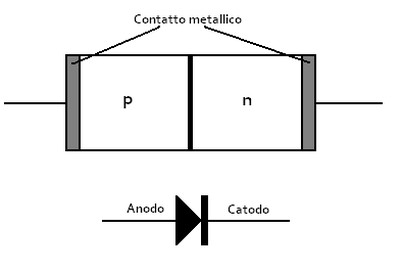
\includegraphics[width=0.5\linewidth]{img/giunz pn.png}
    \end{figure}
\end{definizione}
\subsection{Analisi senza sollecitazioni esterne}
Definiamo $V_{AK}$ e $I_{AK}$ la tensione e la corrente che scorrono tra anodo e catodo senza sollecitazioni esterne, saranno quindi \textbf{nulle}.
\subsubsection{Studio del campo elettrico interno alla Giunzione}
Alla giunzione si avranno elettroni che si spostano da N a P per via delle differenza di concentrazione di questi e, allo stesso tempo, le lacune da N a P andando quindi a combinarsi con gli altri e portando a far scomparire gli elettroni liberi intorno alla zona di giunzione.
Questa prende il nome di \textbf{zona di svuotamento} ($W$)e sarà composta solo da cariche fisse.
\begin{figure}[H]
    \centering
    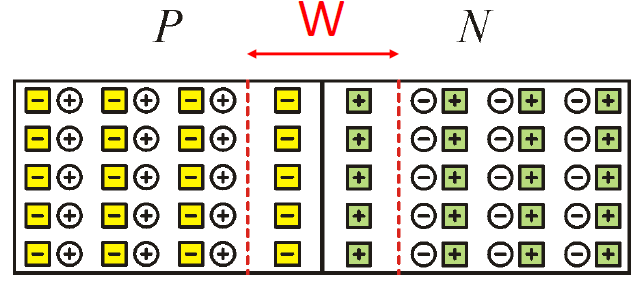
\includegraphics[width=0.5\linewidth]{img/zon svuot.png}
\end{figure}
La differenza delle cariche nella zona di svuotamento da origine a un campo elettrico e quindi a una differenza di potenziale che si oppone alla diffusione di cariche libere, si ha quindi la formazione di una barriera energetica\footnote{Gli elettroni, in quanto cariche negative, sono respinte dal "polo" positivo verso N, le cariche positive sono spinte indietro verso P dal campo elettrico che va proprio verso P}.
La crescita della zona di svuotamento, dal momento della giunzione, è quindi limitata dalla formazione di questa barriera energetica che a un certo punto fermerà altre cariche intente ad attraversarla (contrapposizione tra una piccola corrente di drift e una piccola di diffusione).
\subsubsection{Il potenziale interno}
\begin{definizione}
    [Potenziale interno (o di built-in)]
    Pontenziale ai capi della zona di svuotamento, si indica con $V_0$.
    È quello che impedisce al processo di diffusione di continuare in modo indefinito.
    Calcolabile come
    \[
    V_0 = \frac{kT}{q} \cdot \ln\left(\frac{N_A N_D}{n_i^2}\right)
    \]
\end{definizione}
\subsubsection{La barriera di potenziale}
\subsubsection{Potenziale ai capi del Diodo}
\subsection{Analisi della Giunzione Polarizzata}
\subsubsection{Potenziale positivo}
\subsubsection{Potenziale negativo}
\subsubsection{La giunzione come oggetto rettificante}
La giunzione è un oggetto rettificante in quanto solo quando viene applicata una tensione positiva avrò una corrente da P a N dovuta ai portatori maggioritari, mentre per tensione negativa avrò una corrente da N a P dovuta ai portatori minoritari.
\begin{definizione}
    [Rettificatore]
    Un circuito è detto tale quando trasforma un segnale alternato in uno unidirezionale.
\end{definizione}
\subsubsection{La zona di svuotamento}
\subsubsection{L’equazione di Shockley per la corrente}
$I_{AK}$ viene scelta in verso positivo da P verso N ed è data dall'equazione del modello di Shockley
\[
I_{AK} = I_S(e^{\frac{V_D}{\eta V_T}} - 1)
\]
con $V_T$ tensione termica ai terminali del diodo, $I_S$ corrente inversa di saturazione e $\eta$ fattore di idealità dipendente dai materiali.

\textbf{Concludiamo} che la corrente scorre nel dispositivo in quantità non trascurabile solo se viene applicato ad esso un potenziale positivo tra anodo e catodo, tale da far abbassare la barriera energetica.
In caso di potenziale negativo la corrente è costante e negativa in valore trascurabile.
\begin{figure}[H]
    \centering
    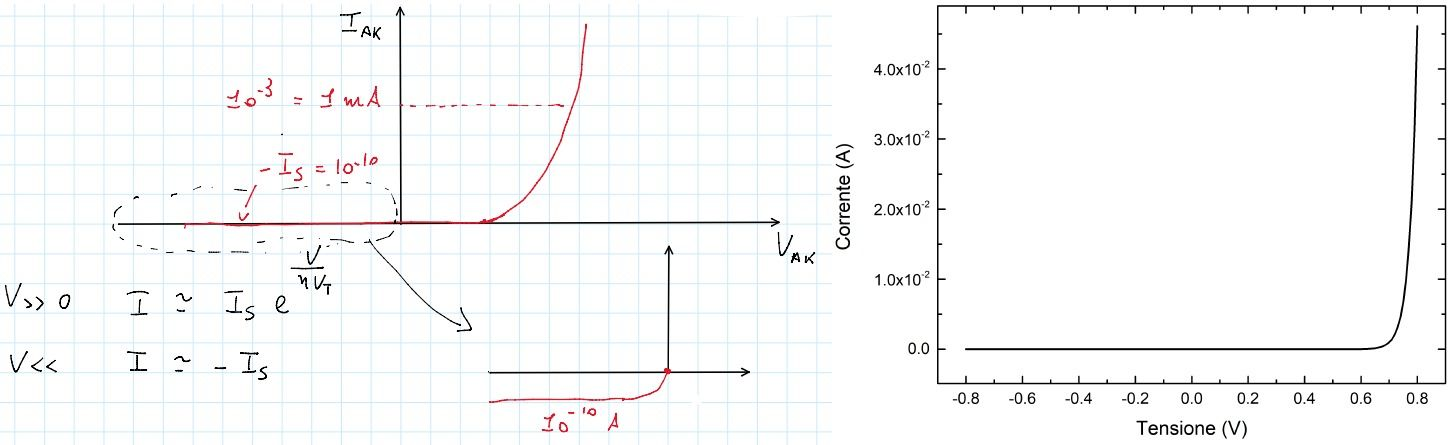
\includegraphics[width=0.75\linewidth]{img/corr diodo.png}
\end{figure}
\subsection{Zone di funzionamento}
Individuano valori di tensione e corrente tipici che risultano in componenti differenti del dispositivo.
Nella giunzione PN, le principali zone di funzionamento sono ($I_D = I_{AK}$):
\begin{itemize}
    \item \textbf{polarizzazione inversa}: $V_D < 0$, il fattore $-1$ nell'equazione è predominante rispetto all'esponenziale, che risulta in $I_D \approx -I_S$. La corrente che scorre è dovuta solamente alle componenti di drift e dunque ai minoritari, il che ci fa capire che essa sia molto piccola;
    \item \textbf{polarizzazione nulla}: $V_D = 0$, la corrente è nulla. Grazie a ciò ricordiamo che l'equazione del modello di Shockley passa per lo $0$;
    \item \textbf{polarizzazione diretta}: $V_D > 0$, la corrente è data dall'esponenziale, che è predominante rispetto al fattore $-1$.
\end{itemize}

\section{Il fenomeno del Breakdown}
c'è in realtà una quarta zona: \textbf{forte inversione}. 
Questa si verifica quando $V_D<<0$ e la corrente inversa aumento in modo repentino. 
\begin{definizione}
    [Breakdown]
    Fenomeno che aumenta il passaggio di portatori attraverso la giunzione.
    Si compone di due fenomeni separati:
    \begin{itemize}
        \item \textbf{Zener}: conseguenza della rottura dei legami covalenti nella zona di svuotamento causata dall'elevato campo elettrico.
        \item \textbf{a valanga}: si verifica quando il campo elettrico nella zona di svuotamento può accelerare i portatori minoritari che attraversano la zona stessa fino a una velocità tale da rompere i legami covalenti degli atomi con cui collidono.
    \end{itemize}
\end{definizione}
\subsection{Effetto Zener}
Si generano nuovi elettroni liberi che trovando campo elettrico favorevole comportano un aumento della corrente.
\subsubsection{Influenza della temperatura sull'effetto Zener}
Alte temperature lo amplificano, a pari corrente la \textbf{tensione di breakdown} ($V_{Br}$) diminuisce.
\subsection{Effetto a valanga}
Si generano nuove coppie \textit{elettrone-lacuna} per via degli urti, processo detto \textbf{ionizzazione dell'atomo}.
\subsubsection{Influenza della temperatura sull'effetto a valanga}
A parità di corrente $V_{Br}$ aumenta.
\subsection{Considerazioni in relazione alla generazione termica}
La generazione termica risulta trascurabile una volta presente il breakdown (anche se i due fenomeni si sommano).

\section{I diodi Zener}
\begin{definizione}
    [Diodo Zener]
    Diodi che permettono il verificarsi del fenomeno del breakdown anche a tensioni con modulo molto basso, nell'ordine della decina di Volt.
    \begin{itemize}
        \item nei diodi con $|V_{Br}| > 7V$, predomina la \textbf{moltiplicazione a valanga}.
        \item nei diodi con $|V_{Br}| < 5V$, predomina l'\textbf{effetto Zener}.
        \item nei diodi in cui $5V < |V_{Br}| < 7V$, si verificano \textbf{entrambi i fenomeni}.
\end{itemize}
\end{definizione}
\subsection{Caso di correnti elevate}
In caso di $V_D>>)$ si hanno correnti \textbf{molto elevate}, non si possono più trascurare gli effetti delle resistenze in serie.
Non possiamo più quindi trascurare le cadute di potenziale nelle zone neutre (zone comprese tra i contatti e la zona di svuotamento).

Questo comporta che all'aumentare della tensione la corrente aumenta meno di quanto ci aspettassimo, il modello di Shockley non è più vero.
\subsection{Simboli circuitali dei diodi di Zener}
\begin{figure}[H]
    \centering
    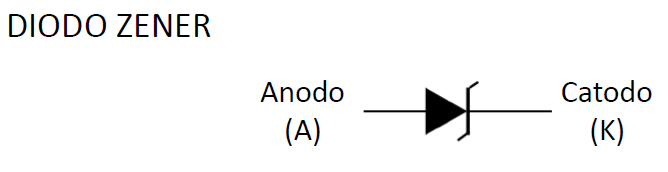
\includegraphics[width=0.5\linewidth]{img/diodo z.png}
\end{figure}

\section{Metodi risolutivi per circuiti con diodi}
Modelli che presentano assunzioni e semplificazioni per la risoluzione dei circuiti
\subsection{Assunzione della tensione}
\begin{figure}[H]
    \centering
    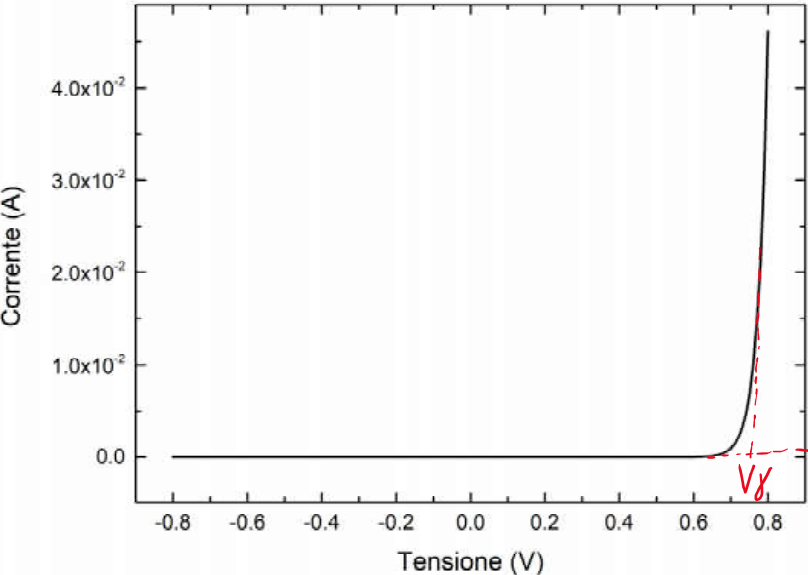
\includegraphics[width=0.5\linewidth]{img/tens corr caratt.png}
    \caption{Grafico Tensione‑Corrente della caratteristica}
\end{figure}
dove $V_\gamma = 0.7V$ ed è la tensione che usiamo come riferimento: per valori inferiori consideriamo che non scorre corrente.
\begin{nota}
    Non consideriamo mai il caso di corrente elevate.
\end{nota}
\subsection{Il modello matematico}
\begin{figure}[H]
    \centering
    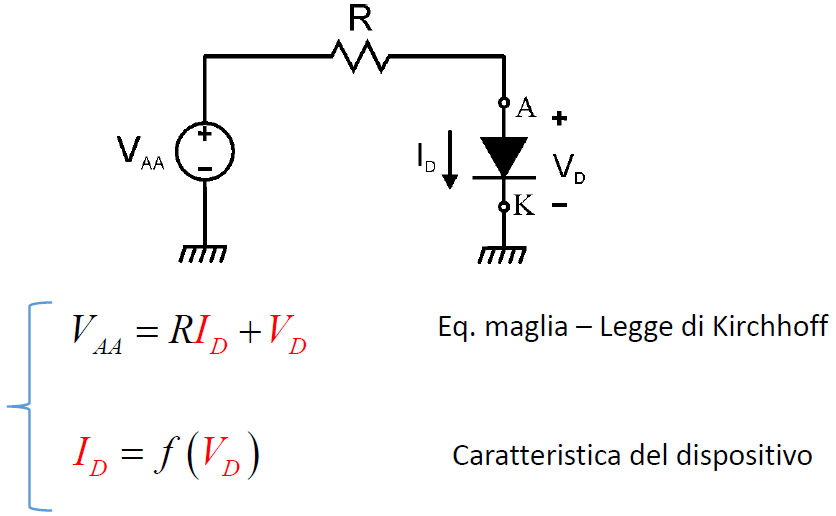
\includegraphics[width=0.38\linewidth]{img/circ es mod mat.png}
\end{figure}
Essendo la corrente passante per il diodo legata all'equazione di Shockley per risolvere il sistema bisogna ricorrere a un metodo iterativo.
\subsection{Metodo Grafico}
Scrivo $I_D$ in funzione di $V_D$ ottenendo una retta a pendenza negativa (\textbf{retta di carico}), e disegnamo in rosso l'equazione trascendente oggetto di studio.
\begin{figure}[H]
    \centering
    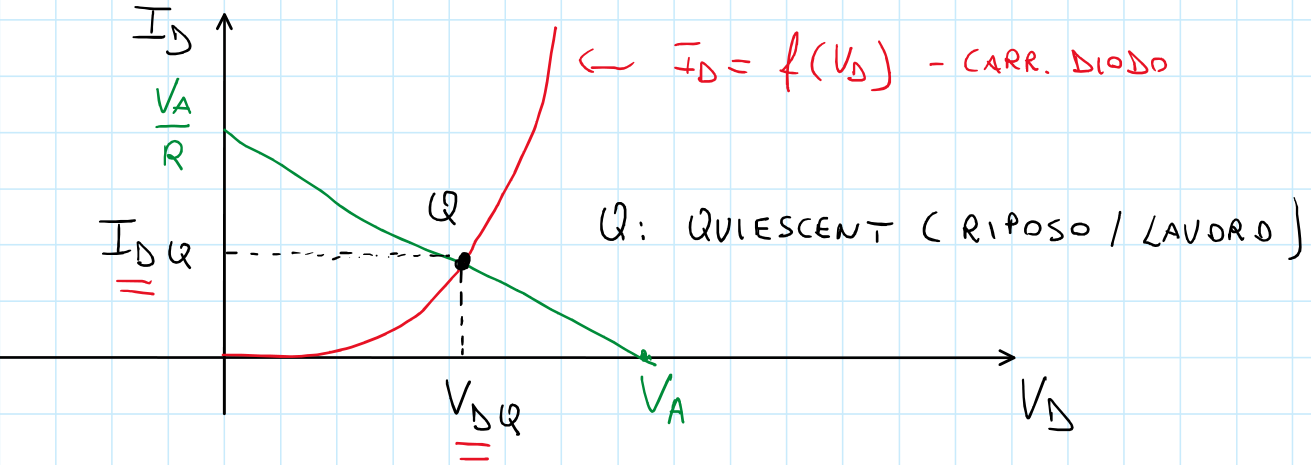
\includegraphics[width=0.5\linewidth]{img/metodo grafico.png}
\end{figure}
L'intersezione tra queste due curve (\textbf{punto Q}) è detta \textbf{punto di lavoro} o \textbf{punto di riposo}.

\begin{itemize}
    \item \textbf{Vantaggi}: metodo non approssimato che permette di visualizzare come si comporta il diodo al variare di alcuni parametri.
    \item \textbf{Svantaggi}: inattuabile in presenza di più diodi, vale solo per quel diodo con quelle specifiche caratteristiche.
\end{itemize}
\subsection{Modelli per grandi segnali}
Metodi che sfruttano un modello approssimato del diodo, rinunciando ad un risultato esatto a fronte di velocità di analisi e piccoli errori.
\subsubsection{Modello a caduta di tensione costante}
Approssima la caratteristica del diodo con una retta verticale, mantenendo $V+\gamma$ e il suo significato. Si può dunque sostituire il diodo con:
\begin{itemize}
    \item un \textbf{generatore di tensione} di valore $V_\gamma$, se $V \geq V_\gamma$;
    \item un \textbf{circuito aperto}, se $V < V_\gamma$.
\end{itemize}
\subsubsection{Modello del diodo ideale}
Considera trascurabile la tensione del diodo: lo semplifica quindi con un interruttore
\begin{figure}[H]
    \centering
    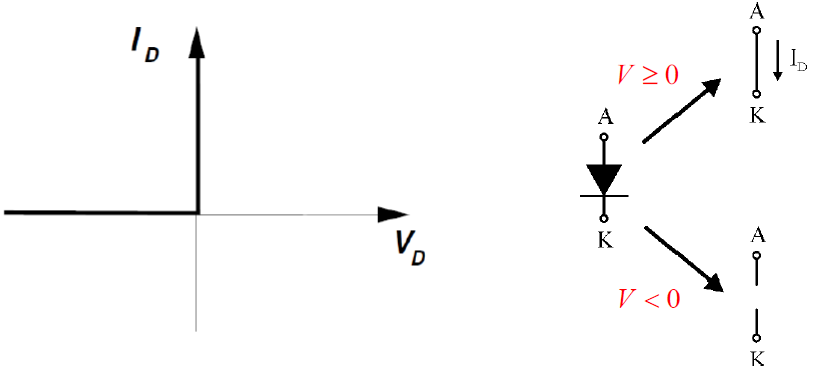
\includegraphics[width=0.5\linewidth]{img/diodo idea.png}
\end{figure}
\begin{nota}
    Continua a valere lo scorrimento di corrente unidirezionale da anodo a catodo.
\end{nota}
\subsubsection{Modello lineare a tratti}
\begin{nota}
    Modello meno approssimato tra quelli per i grandi segnali.
\end{nota}
\begin{itemize}
    \item Caratteristica approssimata con una retta di una certa pendenza
    \item Diodo approssimato con un \textbf{circuito aperto} o con una \textbf{resistenza in serie a un generatore di tensione}
\end{itemize}
\begin{nota}
    Tensione e resistenza della resistenza in serie non noti e approssimati a $R_f=20\Omega$ e $V_f=0.65V$
\end{nota}
\subsection{Esempio di analisi di un circuito con diodi}
Procedura:
\begin{itemize}
    \item ipotizzo lo stato di ciascun diodo: \textbf{conduzione} o \textbf{interdizione}
    \item Sostituisco ciascun diodo con il modello corrispondente;
    \item Risolvo il circuito semplificato;
    \item Verifico la correttezza delle ipotesi iniziali per \textbf{ciascun diodo}:
    \begin{itemize}
        \item se tutte sono verificate, allora ho ottenuto una soluzione corretta;
        \item se anche solo una delle ipotesi è errata, allora bisogna cambiare l'ipotesi, risolvere nuovamente il circuito e ri-verificare la correttezza della nuova ipotesi, fino ad ottenere un risultato accettabile
    \end{itemize}
\end{itemize}
\begin{figure}[H]
    \centering
    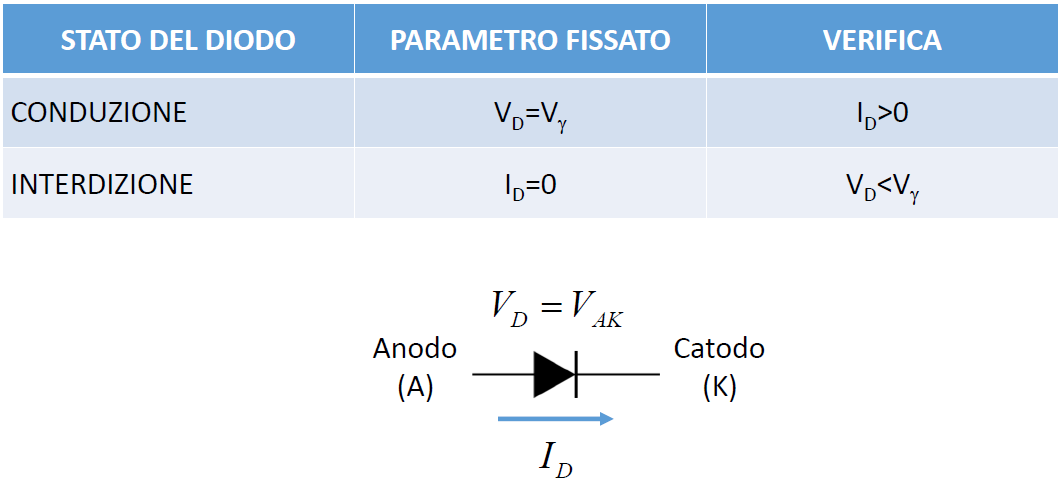
\includegraphics[width=0.5\linewidth]{img/param verifica.png}
\end{figure}
\subsubsection{Risoluzione con modello a caduta di tensione costante}
\subsubsection{Risoluzione con modello del diodo ideale}
\subsubsection{Risoluzione con modello lineare a tratti}
\subsection{Considerazioni sull'efficacia dei modelli}
\begin{figure}[H]
    \centering
    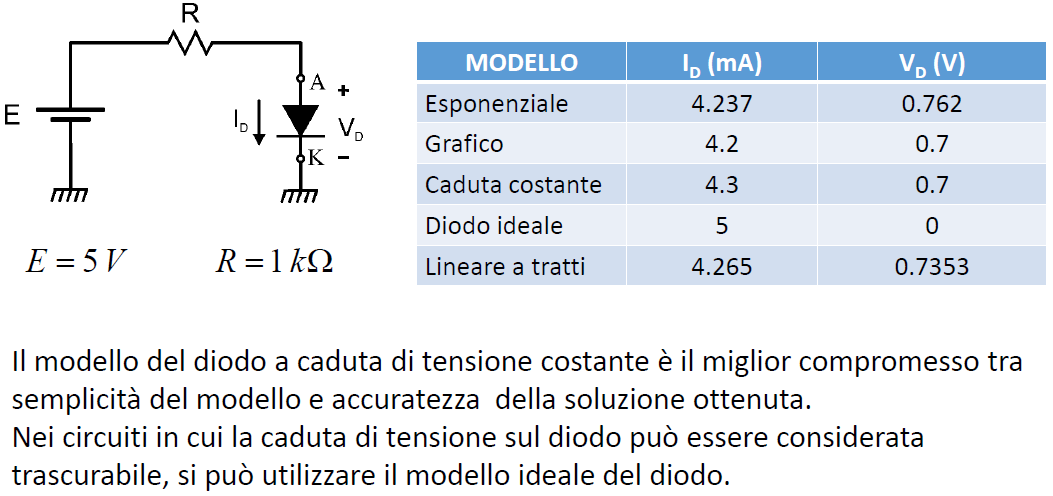
\includegraphics[width=0.5\linewidth]{img/efficacia modelli.png}
\end{figure}
recap

\section{Circuiti con diodi}
Circuiti che sfruttano i diodi per ottenere una tensione continua partendo da quella alternata.
\subsection{Circuito rettificatore}
Chiamato anche \textbf{circuito a raddrizzatore di singola semi-onda}: blocca la tensione negativa
\begin{figure}[H]
    \centering
    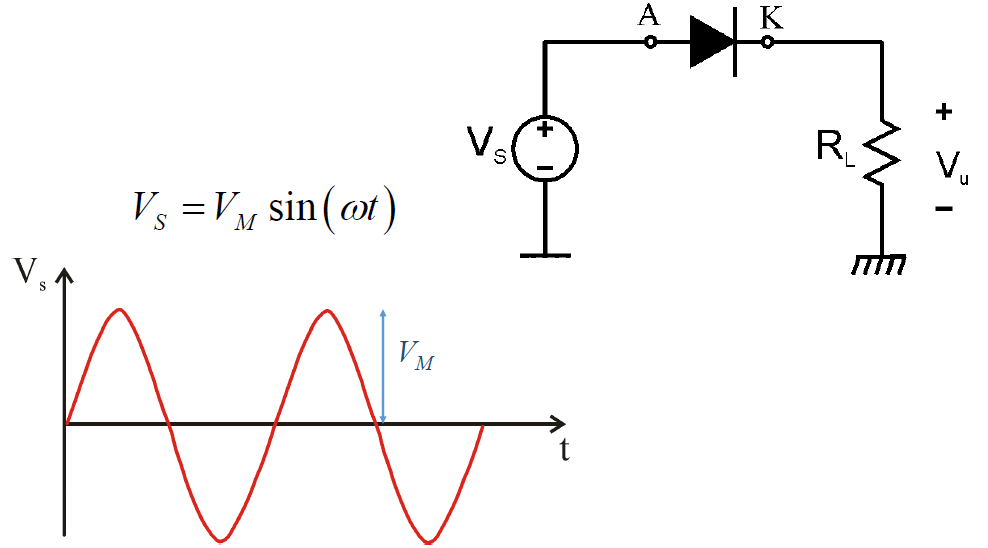
\includegraphics[width=0.5\linewidth]{img/circ rettificatore.png}
\end{figure}

\subsection{Il PIV}
Circuito che funziona correttamente solo se il diodo rimane \textbf{interdetto} per tutto l'intervallo di non conduzione.
\textbf{Attenzione} al caso in cui la tensione inversa supera un certo valore e porta il diodo in \textbf{breakdown} e quindi a condurre corrente non più trascurabile.
\begin{definizione}
    [PIV]
    Il Peak Inverse Voltage è il parametro che tiene conto della tensione inversa massima applicata al diodo prima che vada in \textbf{breakdown}.
    \begin{nota}
        Nel caso del circuito rettificatore $PIV = V_M$ dove \textbf{$V_M$} indica la \textbf{tensione di picco in ingresso}.
    \end{nota}
\end{definizione}
\subsection{Rilevatore di picco ideale}
\begin{figure}[H]
    \centering
    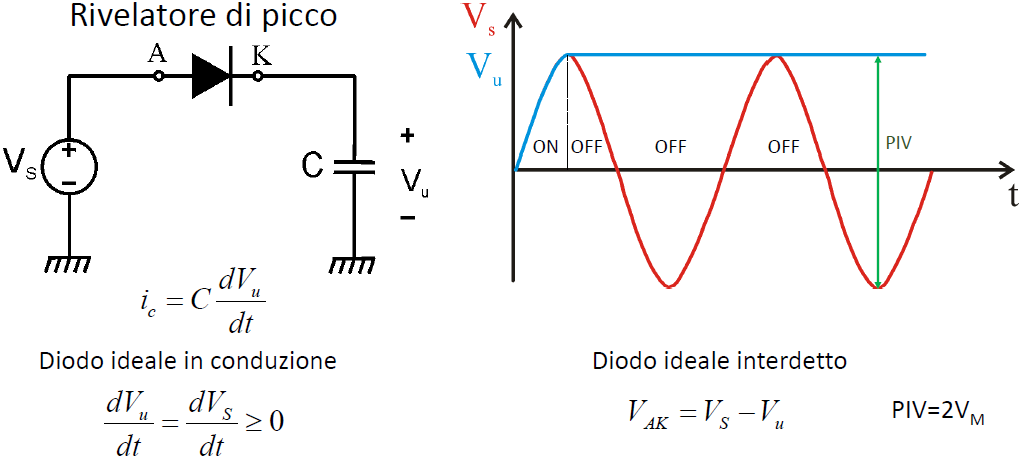
\includegraphics[width=0.5\linewidth]{img/Rilevatore di picco ideale.png}
\end{figure}
\subsection{Circuito rettificatore con filtro RC}
\begin{figure}[H]
    \centering
    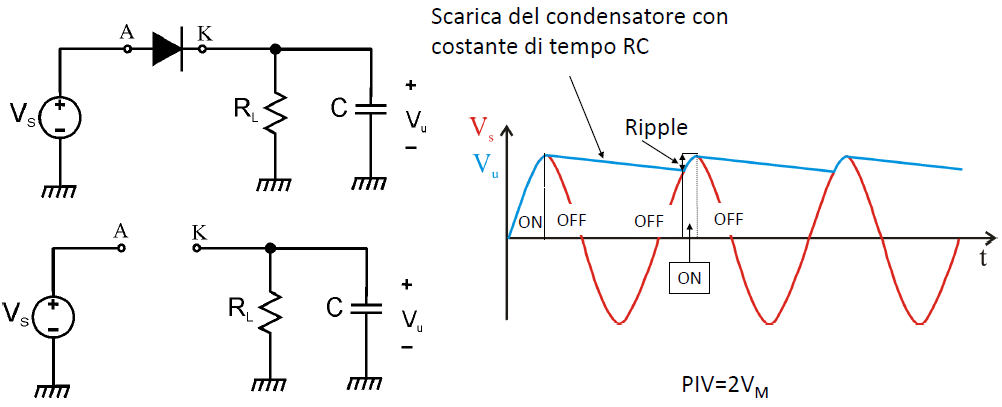
\includegraphics[width=0.5\linewidth]{img/Circuito rettificatore con filtro RC.png}
\end{figure}
\begin{definizione}
    [Ripple]
    Oscillazione della tensione del condensatore nel circuito rettificatore con filtro RC, data dalla differenza tra la tensione di picco e quella minima al condensatore
    \begin{nota}
        PIV si può approssimare al valore di $2V_M$
    \end{nota}
\end{definizione}

\section{Circuiti con trasformatori}
\begin{definizione}
    [Trasformatore]
    Dispositivo che permette di trasformare una tensione in un'altra mantenendo la stessa corrente.
\end{definizione}
\subsection{Raddrizzatore a doppia semi-onda}
\begin{definizione}
    [Raddrizzatore a doppia semi-onda]
    Circuito che permette invertire il lobo negativo della tensione sinusoidale, ottenendone uno positivo.
\end{definizione}
\subsubsection{Raddrizzatore a doppia semi‑onda con trasformatore a presa centrale}
\begin{definizione}
    [Raddrizzatore a doppia semi‑onda con trasformatore a presa centrale]
    Tipologia di raddrizzatore in cui il condensatore è assente.
    \begin{figure}[H]
        \centering
        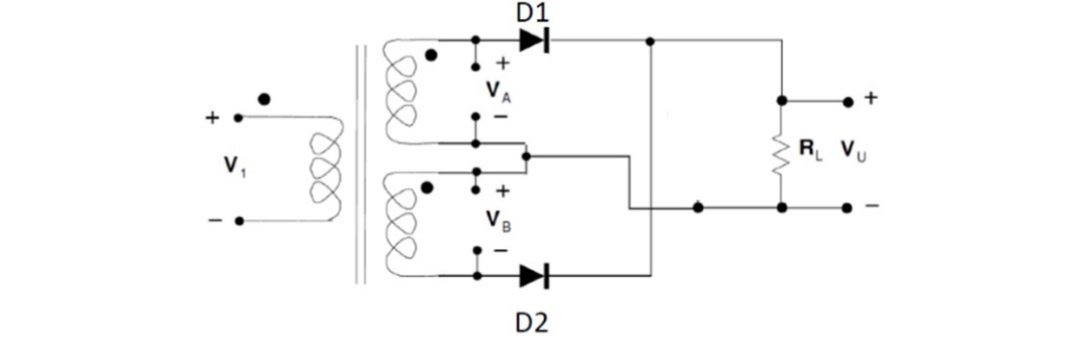
\includegraphics[width=0.75\linewidth]{img/raddr presa centra.png}
    \end{figure}
\end{definizione}
\paragraph{Primo semi-periodo}
\paragraph{Secondo semi-periodo}
\paragraph{Conclusioni}
$\s$
\begin{figure}[H]
    \centering
    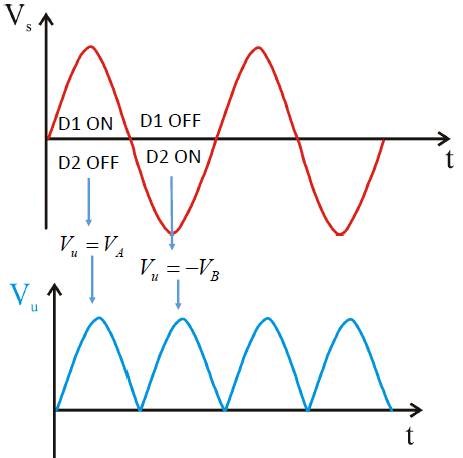
\includegraphics[width=0.3\linewidth]{img/raddr dop sem ond.png}
\end{figure}

\subsubsection{Raddrizzatore a doppia semi‑onda con condensatore}
\begin{definizione}
    [Raddrizzatore a doppia semi‑onda con condensatore]
    Tipologia di raddrizzatore in cui è presente il condensatore.
\end{definizione}
\begin{figure}[H]
    \centering
    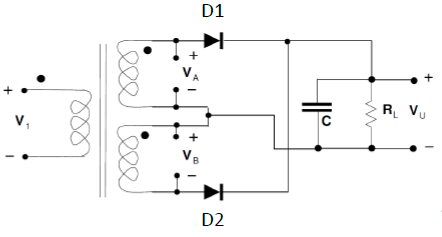
\includegraphics[width=0.5\linewidth]{img/rad do se cond.png}
\end{figure}
\paragraph{Funzionamento}
Comportamento del circuito \textbf{identico} a quello a presa centrale.
Differenza dopo il picco di tensione: il periodo di scarica dura la metà rispetto al circuito rettificatore.
\begin{figure}[H]
    \centering
    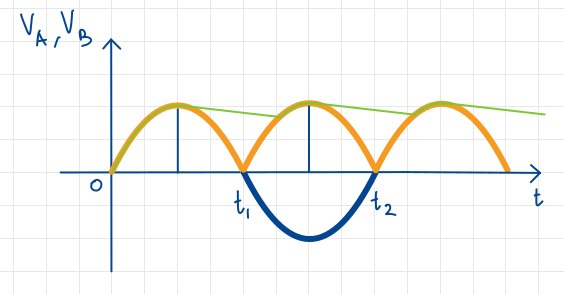
\includegraphics[width=0.25\linewidth]{img/grafico scarica raddr.png}
\end{figure}
\subsection{Raddrizzatore a ponte di Graetz}
\begin{definizione}
    [Raddrizzatore a ponte di Graetz]
    Dispositivo che raddrizza la tensione alternata senza bisogno del doppio circuito secondario: fa in modo che la tensione in uscita abbia sempre lo stesso verso.
    \begin{figure}[H]
        \centering
        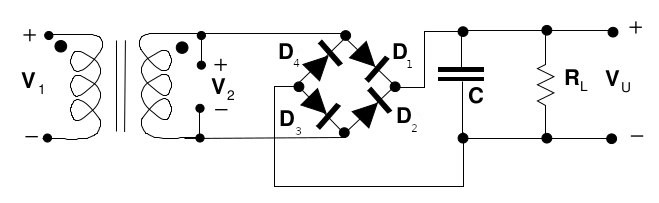
\includegraphics[width=0.75\linewidth]{img/graetz.png}
    \end{figure}
\end{definizione}

\section{I regolatori di tensione}
\begin{definizione}
    [Regolatore di tensione]
    $\s$
    \begin{itemize}
        \item Dispositivo che rende costante la corrente, eliminando i ripple e permettendo di applicare filtri alla tensione.
        \item Dispositivo che in ingresso ha una tensione assimilabile ad una costante con qualche variazione, come quella in uscita da un ponte di Graetz, e in uscita ha una tensione costante.
    \end{itemize}
\end{definizione}
\subsection{Regolatori di tensione Zener}
\begin{definizione}
    [Regolatore di tensione Zener]
    Circuito che utilizza un diodo Zener per regolare la tensione.
    \begin{figure}[H]
        \centering
        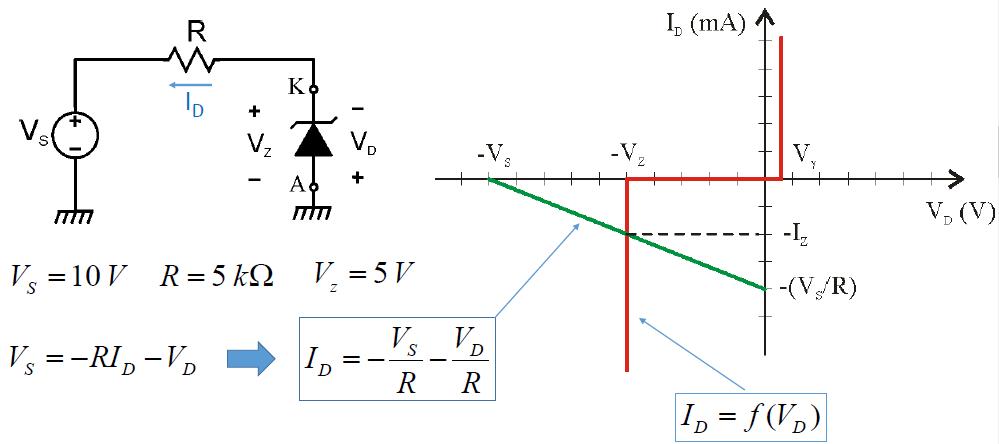
\includegraphics[width=0.5\linewidth]{img/reg tens zener.png}
    \end{figure}
    \begin{nota}
        In questo il diodo è montato al contrario e quindi potrà essere solo spento o in breakdown.
    \end{nota}
\end{definizione}
\subsection{Circuito regolatore Zener}
\begin{definizione}
    [Circuito regolatore Zener]
    Circuito simile al ponte di Graetz ma con in aggiunta un diodo Zener e una resistenza.
    \begin{figure}[H]
        \centering
        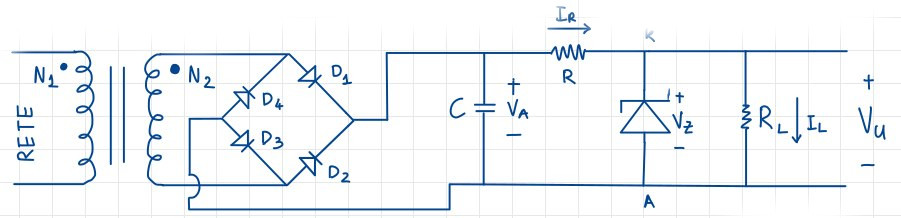
\includegraphics[width=0.75\linewidth]{img/circ reg Z.png}
    \end{figure}
    In questo circuito il diodo Zener assorbe le variazioni di corrente per mantenere $I_L$ costante.
    \begin{nota}
        Per ottenere questo effetto bisogna fare in modo che $I_Z$ rimanga sempre positiva, si hanno quindi limiti sul carico $R_L$.
    \end{nota}
\end{definizione}
\subsubsection{Limiti di funzionamento di corrente}
Limite per il quale il diodo Zener smette di funzionare:
\[
I_Z = 0 \to I_{LMax} = \frac{V_A - V_Z}{R_L}
\]
\subsubsection{Limiti di funzionamento di Potenza}
Valore massimo di potenza sopportabile
\[
P_{ZMax} = I_{ZMax}V_Z = V_Z \frac{V_A - V_Z}{R_L}
\]

\section{La logica a diodi}
La logica a diodi ha come obbiettivo il realizzare circuiti digitali tramite i diodi: scegliamo una tensione di riferimento ($5V$), che indichiamo con ${V_DD}$, a cui assegniamo il valore logico $1$ mentre il valore logico $0$ va alla tensione $0$.
\begin{nota}
    Per entrambi i valori consideriamo una tolleranza, rispettivamente:
    \item $V_{LMin}$
    \item $V_{LMax}$
\end{nota}

\subsection{Circuiti logici}
\subsubsection{Circuito per la porta AND}
\begin{figure}[H]
    \centering
    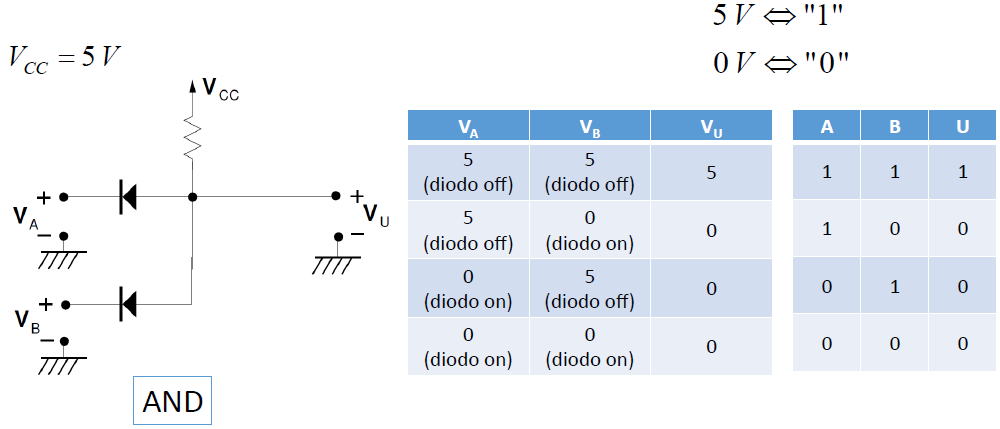
\includegraphics[width=0.5\linewidth]{img/circ and.png}
\end{figure}
\subsubsection{Circuito per la porta OR}
\begin{figure}[H]
    \centering
    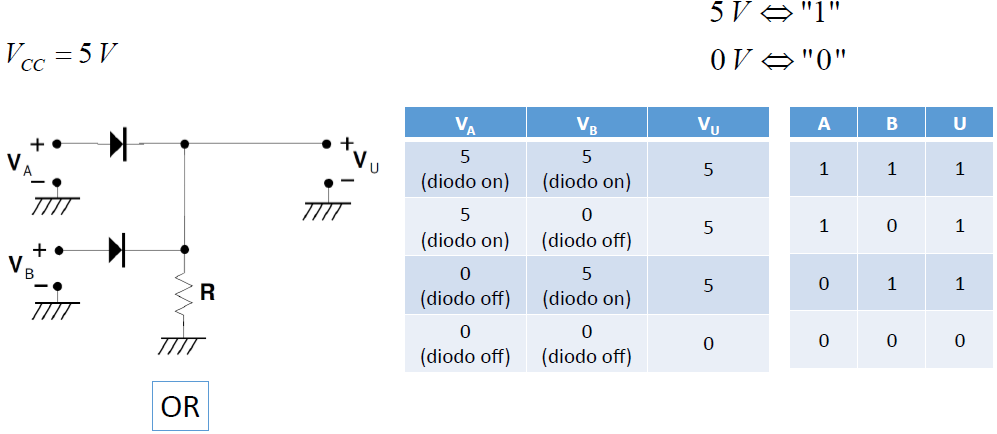
\includegraphics[width=0.5\linewidth]{img/circ or.png}
\end{figure}
\subsection{Problematiche della logica a diodi}
Necessità di molta corrente, degradazione dei livelli logici per più circuiti in cascata, impossibilità di costruire circuiti NOT.

\section{Il modello per i piccoli segnali}
Trattiamo un circuito in presenza di un valore di tensione grande e costante e uno piccolo e variabile.
Per farlo introduciamo delle convenzioni:
\begin{itemize}
    \item Valori \textbf{costanti} scritti come: $V_{CC}$
    \item Valori \textbf{variabili} scritti come: $v_{be}$
    \item Valori \textbf{istantanei o complessivi} scritti come: $v_{BE}$
\end{itemize}
Risolvendo graficamente\footnote{Gli altri metodi non sono più validi} un circuito di questo tipo otteniamo che il punto di riposo varierà lungo la caratteristica e che quindi una piccola variazione del segnale in ingresso può portare a una variazione di esso.
Si approssima pertanto l'esponenziale con una retta (quindi come elemento circuitale si sceglie una \textbf{resistenza} detta \textbf{differenziale} e indicata con $r_d=\text{valore della pendenza della rette nell'interno di Q}$).
\subsection{Risoluzione del primo circuito}
Si dovranno risolvere due circuiti: uno solo con il generatore di tensione e uno in cui, una volta noto Q, calcolo la resistenza differenziale da sostituire al diodo.
\begin{figure}[H]
    \centering
    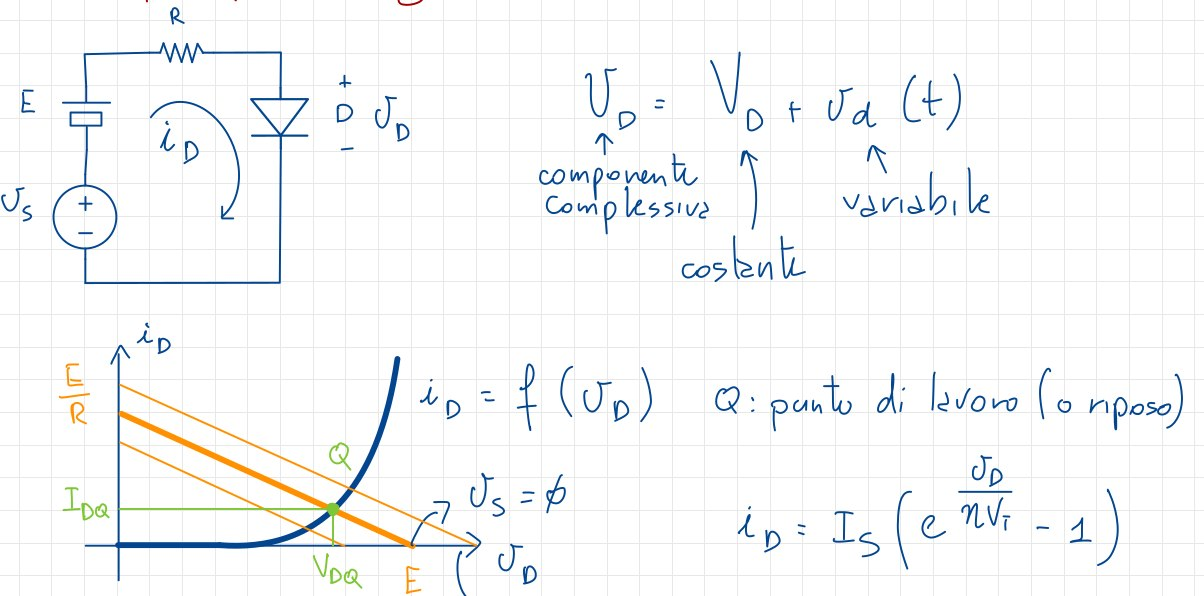
\includegraphics[width=0.5\linewidth]{img/circ pic segn.png}
    \caption{Notare i due generatori di tensione: quello grande e costante (E) e quello piccolo e variabile (v\_s(t)).}
\end{figure}
Primo passo: determinare il punto di riposo.
Per farlo utilizziamo il circuito "in continua":
\begin{figure}[H]
    \centering
    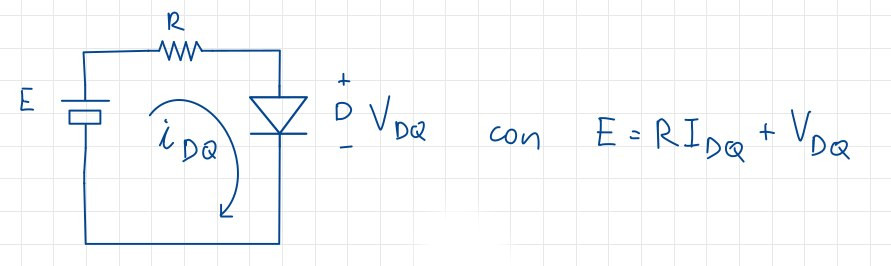
\includegraphics[width=0.35\linewidth]{img/circ in cont.png}
\end{figure}
da cui otteniamo $v_s=Ri_d+v_d$ che è un circuito con due generatori di segnali non costanti ($v_s$ e il diodo $v_d$).
Non potendo usare Shockley (non siamo allo zero ma al punto Q) approssimiamo tramite lo sviluppo in serie che, fermandoci al primo ordine ci da
\[
i_D = \left.\frac{di_D}{dv_D}\right|_{Q}v_d
\] ovvero la relazione tra $i_D$ e $v_D$ cercata.

Definiamo poi la \textbf{conduttanza differenziale} come
\[
g_d = \left.\frac{di_D}{dv_D}\right|_Q
\]
che ci permette di definire la \textbf{resistenza differenziale}
\[
r_d = \frac{1}{g_d}
\]
quindi in prima approssimazione avremo un circuito lineare, che sappiamo risolvere:
\begin{figure}[H]
    \centering
    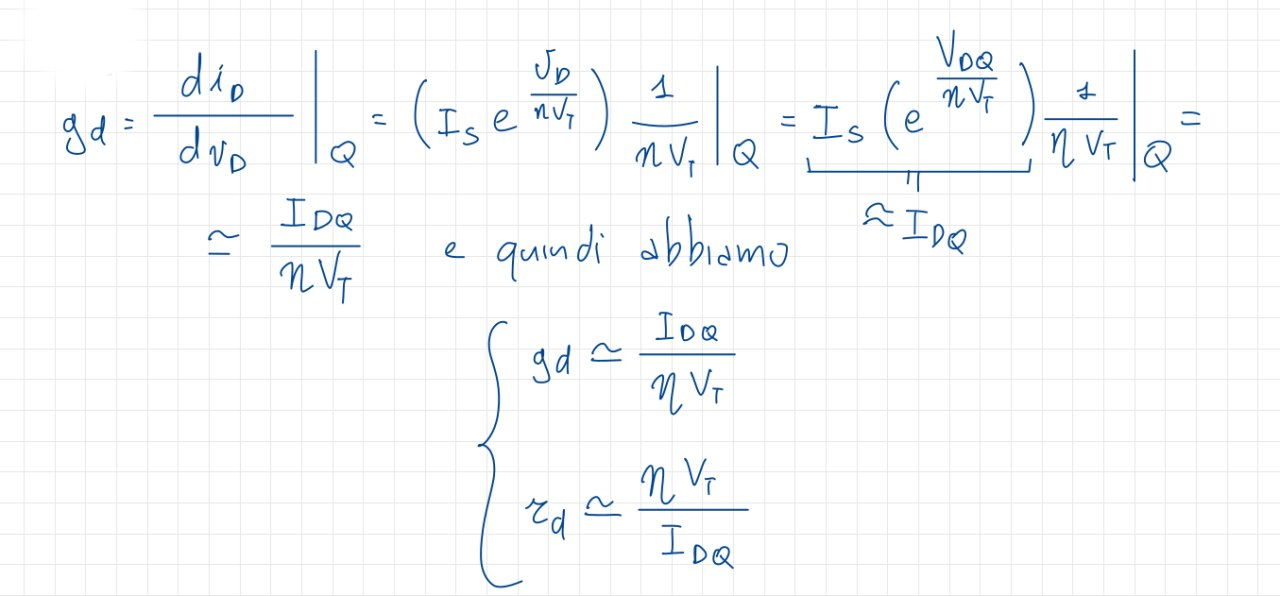
\includegraphics[width=0.5\linewidth]{img/ris circ app.png}
\end{figure}
Con ulteriori calcoli vediamo come per applicare il modello dei piccoli segnali è necessario che la tensione ai capi del diodo sia molto inferiore a $52mV$.

\section{I BJT - Transistor a giunzione bipolare}

\subsection{Generatore di corrente controllato in corrente}
\begin{definizione}
    [Generatore controllato]
    Dispositivo a due porte, quindi con quattro terminali, che si riducono tuttavia nella maggior parte dei casi a tre, perché due sono in comune tra ingresso e uscita.
\end{definizione}
\begin{figure}[H]
    \centering
    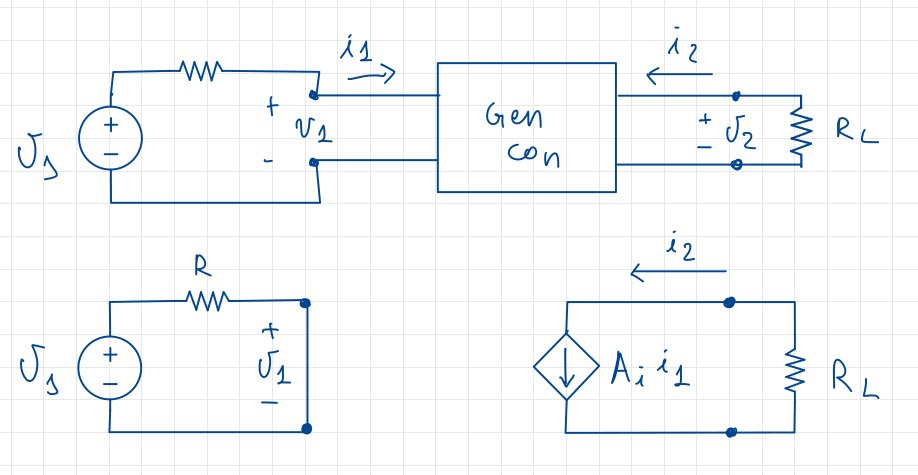
\includegraphics[width=0.5\linewidth]{img/gen cor contr cor.png}
\end{figure}
Dal disegno notiamo che $i_2=A_ii_1$ e quindi definiamo \textbf{guadagno di corrente} $A_i=\frac{i_2}{i_1}$, in particolare:
\begin{itemize}
    \item \textbf{amplificatore di corrente} se $A_i > 1$
    \item \textbf{attenuatore di corrente} se $A_i < 1$
\end{itemize}
Relazioni tra le tensioni e le correnti generate dal generatore:
\[
\begin{cases}
v_2 = -R_L i_2 = -R_L A_i i_1 \\
i_1 = \frac{v_s}{R}
\end{cases}
\to v_2 = \frac{R_L A_i v_s}{R}
\]
\textbf{Guadagno di tensione}: $A_v=\frac{v_2}{v_1}$ per cui possiamo dire:
\begin{itemize}
    \item \textbf{amplificatore di tensione} se $A_v > 1$
    \item \textbf{attenuatore di tensione} se $A_v < 1$
\end{itemize}
\textbf{Guadagno di potenza}:
\[
A_p = \frac{\text{Potenza sul carico}}{\text{Potenza in ingresso}} = -\frac{v_2 i_2}{v_s i_1} = -A_v A_i
\]
che, una volta sviluppata la relazione, notiamo essere \textbf{sempre positivo}.
\subsubsection{Caratteristiche del circuito}
\begin{itemize}
    \item \textbf{di ingresso}: rappresentazione del comportamento sul piano $i_1, v_1$
    \item \textbf{di uscita}: rappresentazione del comportamento sul piano $i_2, v_2$
\end{itemize}
Notiamo che la caratteristica in ingresso non ha alcuna dipendenza da quella in uscita mentre quella in uscita è legata all'altra vista la relazione $i_2=A_ii_1$.

\subsection{BJT}
\subsubsection{Intro}
Il transistore bipolare è, dal punto di vista fisico, un dispositivo con due giunzioni PN poste una di seguito all'altra, ma orientate in senso opposto: a seconda di come lo costruiamo, potremo avere dunque due tipi di transitori bipolari: \textbf{PNP} e \textbf{NPN}.
\begin{figure}[H]
    \centering
    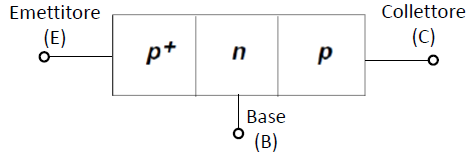
\includegraphics[width=0.5\linewidth]{img/schema bjt.png}
    \caption{Schema BJT}
\end{figure}
Il transistor per funzionare necessita che una delle due estremità abbia un drogaggio maggiore dell'altra, indicato con $+$.
Il dispositivo ha poi 3 terminali:
\begin{itemize}
    \item \textbf{emettitore}, che corrisponde all'estremo maggiormente drogato;
    \item \textbf{collettore}, che corrisponde all'estremo meno drogato;
    \item \textbf{base}, che corrisponde all'estremo intermedio, a comune tra i due dispositivi.
\end{itemize}
Simbolo circuitale (la freccia indica l'emettitore):
\begin{figure}[H]
    \centering
    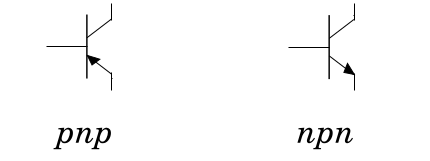
\includegraphics[width=0.5\linewidth]{img/trans.png}
\end{figure}
\subsubsection{Zona di funzionamento in Zona Attiva Diretta}
Ci concentriamo sulla zona di funzionamento maggiormente utilizzata in ambito analogico: in questa la giunzione base-emettitore è polarizzata in diretta mentre quella base-collettore in inversa.
\begin{figure}[H]
    \centering
    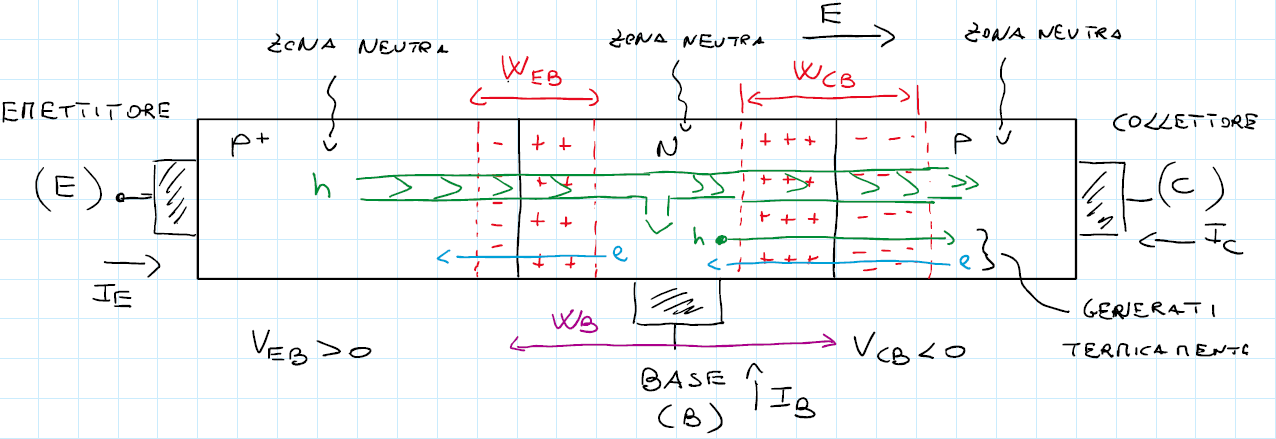
\includegraphics[width=0.5\linewidth]{img/spost car el.png}
    \caption{Schema degli spostamenti di lacune ed elettroni}
\end{figure}
Tra base ed emettitore si ha una grande, per via del maggiore drogaggio dell'emettitore, iniezione di lacune e una trascurabile diffusione di elettroni da $N$ verso $P^+$.

Assunzione \textbf{importante}: campo elettrico nelle zone neutre piccolo, quindi spostamento di cariche solo per diffusione.

Si nota poi come le lacune iniettate da $P^+$ verso $N$ si ritrovino in un semiconduttore drogato $N$ e quindi si combinano facilmente con elettroni, se non fosse che la base è molto piccola quindi la maggior parte delle lacune arriverà alla zona $W_{CB}$ dove il campo favorevole trascina le lacune verso il collettore: si ha quindi una transizione di portatori (di lacune) da emettitore a collettore.
\begin{nota}
    Condizioni di funzionamento del BJT in ZAD: drogaggio base piccola e stretta, giunzione base collettore tale che la corrente in essa sia trascurabile, portatori nella zona neutra mossi solo per diffusione.
\end{nota}
Si ottiene che la corrente che scorre dall'emettitore al collettore è \textbf{costante} e \textbf{controllabile tramite la corrente di base} (questa è infatti la grandezza pilota del sistema).
La corrente di base rifornisce la stessa di elettroni che altrimenti verrebbero persi per via della ricombinazione (che porterebbero la base a carica positiva e ostacolerebbe l'iniezione di lacune) e quelli che per diffusione vanno nell'emettitore.
Notiamo che: dato che la \textbf{percentuale di lacune perse nella ricombinazione è fissa} allora se aumentiamo la corrente di base aumenta anche quella da emettitore a collettore (\textbf{flusso principale}).
\begin{nota}
    la corrente di ricombinazione è piccola quindi quella di base è piccola rispetto a quella controllate quindi \textbf{BJT è un amplificatore di corrente}.
\end{nota}
\subsubsection{Modello di Ebers-Moll}
Per evitare la trattazione matematica, utilizzeremo il modello di Ebers‑Moll per grandi segnali del transistore.
\begin{figure}[H]
    \centering
    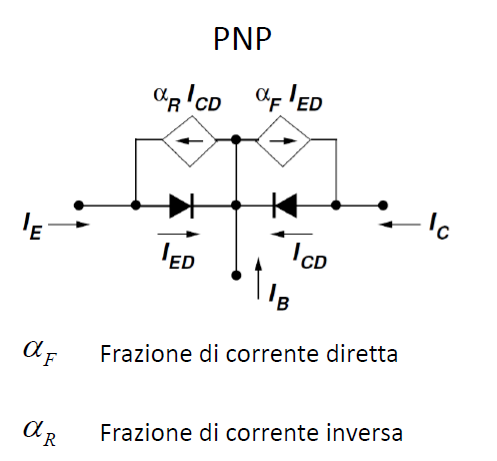
\includegraphics[width=0.5\linewidth]{img/eb mol.png}
    \caption{Circuito equivalente di un BJT}
\end{figure}
In polarizzazione diretta le lacune che riesco a passare dall'emettitore al collettore sono date dal generatore controllato $\alpha_F I_{ED}$. Con $\alpha_F$ (forward) indichiamo la \textbf{frazione di corrente diretta}, ovvero la frazione di portatori iniettati dall'emettitore in Base che riescono ad arrivare al Collettore.
È un valore tra 0.98 e 0.988, il mancante è dovuto alle ricombinazioni.

Il transistor può lavorare anche in polarizzazione inversa (generatore controllato e corrente $CD$). In questo caso $\alpha_R$ (reverse) indica la \textbf{frazione di corrente inversa} ed è compresa tra 0.4 e 0.8 (è quindi meno efficace, questo per via dei drogaggi).
\subsubsection{Equazioni di Ebers-Moll}
\begin{figure}[H]
    \centering
    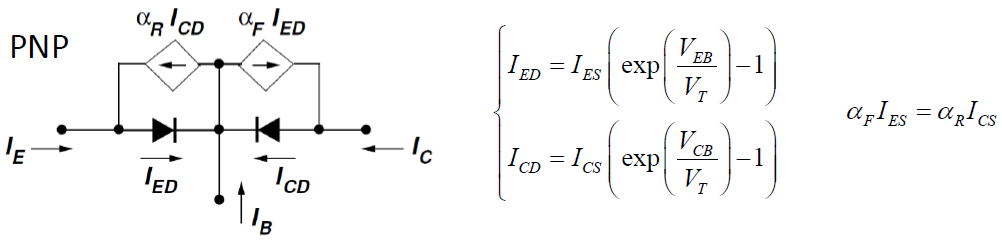
\includegraphics[width=0.75\linewidth]{img/eq eb mol.png}
\end{figure}
\textbf{Regola di reciprocità} $\alpha_F I_{ES} = \alpha_R I_{CS}$.
\subsubsection{Riepilogo}
\begin{figure}[H]
    \centering
    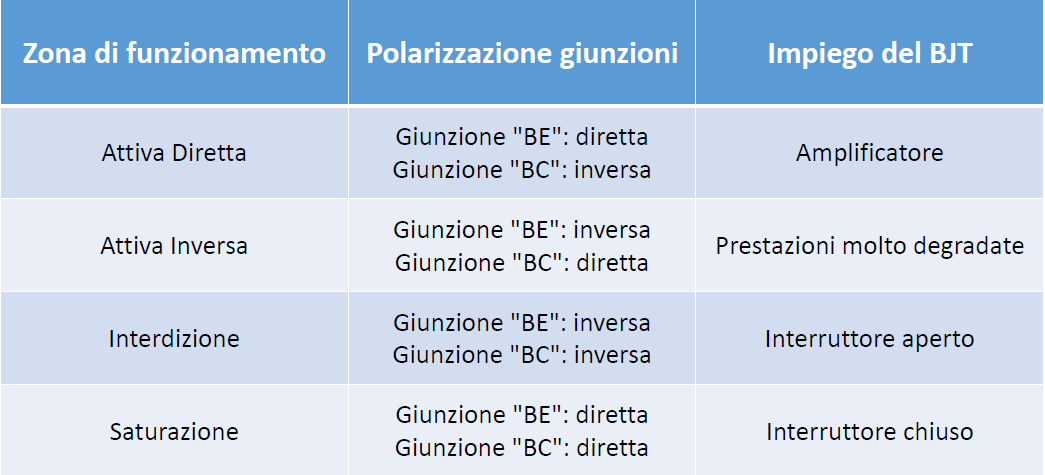
\includegraphics[width=0.5\linewidth]{img/recap bjt.png}
\end{figure}
\subsubsection{Struttura fisica del BJT PNP}
Qui possiamo notare come \textbf{non} sia \textbf{simmetrico}.
\begin{figure}[H]
    \centering
    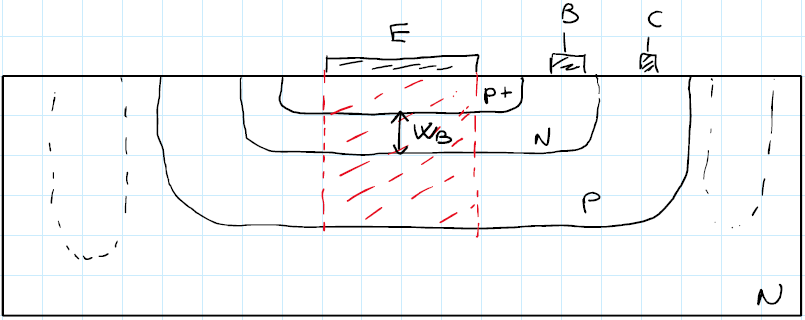
\includegraphics[width=0.5\linewidth]{img/fisic bjt.png}
\end{figure}
\subsection{BJT NPN}
Per rendere il transistor un dispositivo solo con una porta di ingresso e una di uscita colleghiamo in comune uno dei tre terminali.
Ci concentriamo solo sul caso a emettitore comune: il terminale dell'emettitore è collegato in comune tra ingresso e uscita.
\begin{figure}
    \centering
    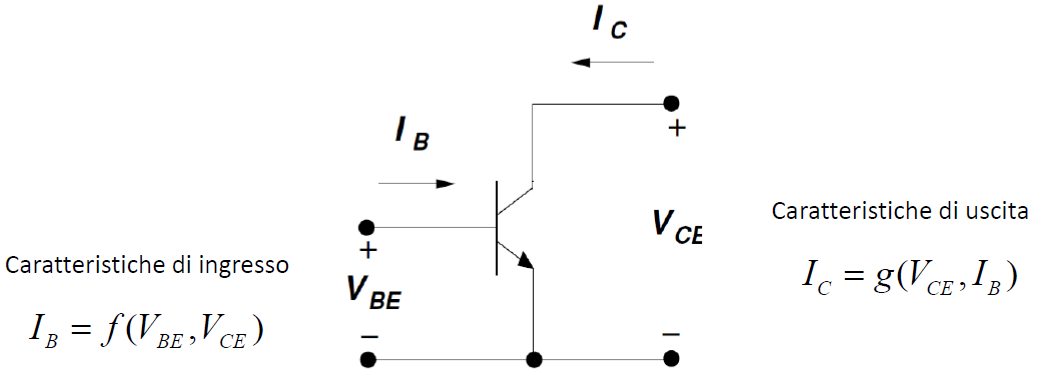
\includegraphics[width=0.5\linewidth]{img/bjt npn.png}
    \caption{Circuiti di configurazione a emettitore comune}
\end{figure}
Per il nostro studio, considereremo solo il transistor NPN, in cui gli elettroni si muovono dall'emettitore al collettore e le lacune si muovono dalla base all'emettitore. In questo modo, avremo una corrente che scorre dal collettore all'emettitore e un flusso di lacune nella base.

Specifiche del modello:
\begin{itemize}
    \item \textbf{ingresso}: corrente di base $I_B$ in funzione di $V_{BE}$ e $V_{CE}$
    \item \textbf{uscita}: corrente di collettore $I_C$ in funzione di $I_B$ e $V_{CE}$
\end{itemize}
\subsubsection{Modello di Ebers-Moll per il transistor NPN}
\begin{figure}[H]
    \centering
    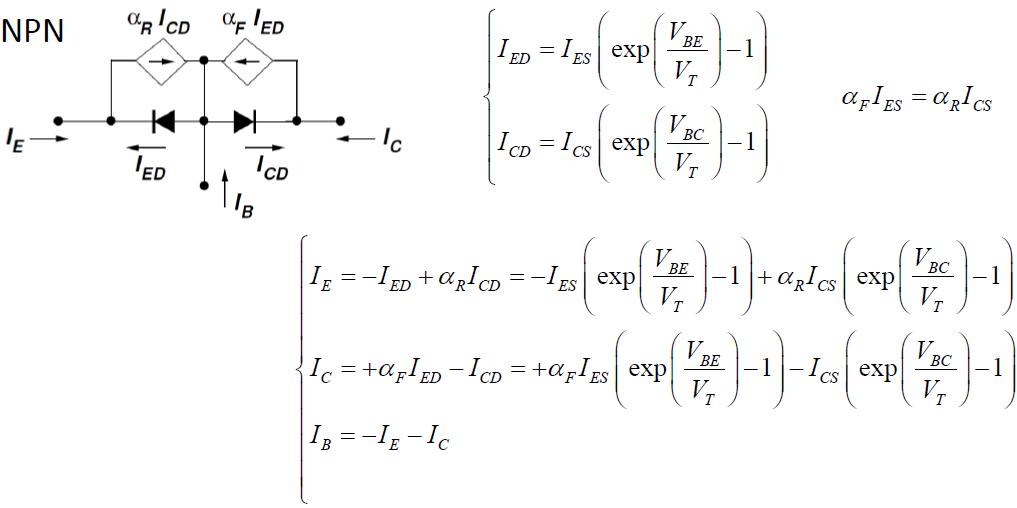
\includegraphics[width=0.75\linewidth]{img/eb per npn.png}
\end{figure}
Siamo nel caso di un generatore di corrente controllato in corrente.

...

Si ottiene infine che la corrente di uscita non dipende dalla tensione ma da $\beta_F$ detto \textbf{guadagno di corrente in cortocircuito a emettitore comune} compreso tra 200 e 300, questi valori alti ci suggeriscono che basta un piccola corrente di base per controllare una grande corrente di collettore.
\subsubsection{Caratteristiche di uscita}
$I_B$ proporzionale alla $I_C$ per un fattore $\beta_F$.
Questo vale solo per valori di $V_CE$ non troppo piccoli, altrimenti le caratteristiche collassano diminuendo la corrente del collettore.
Ne concludiamo che $V_CE$ influenza la caratteristica di uscita mandando in dispositivo in \textbf{saturazione}.
\subsubsection{Caratteristiche di ingresso}
\[
I_B = (1 - \alpha_F)I_{ES} \cdot e^{\frac{V_{BE}}{V_T}}
\]
La corrente di base è dipendente dalla tensione in ingresso: la caratteristica di uscita avrà un andamento esponenziale.
\subsection{Effetto Early}
\begin{figure}[H]
    \centering
    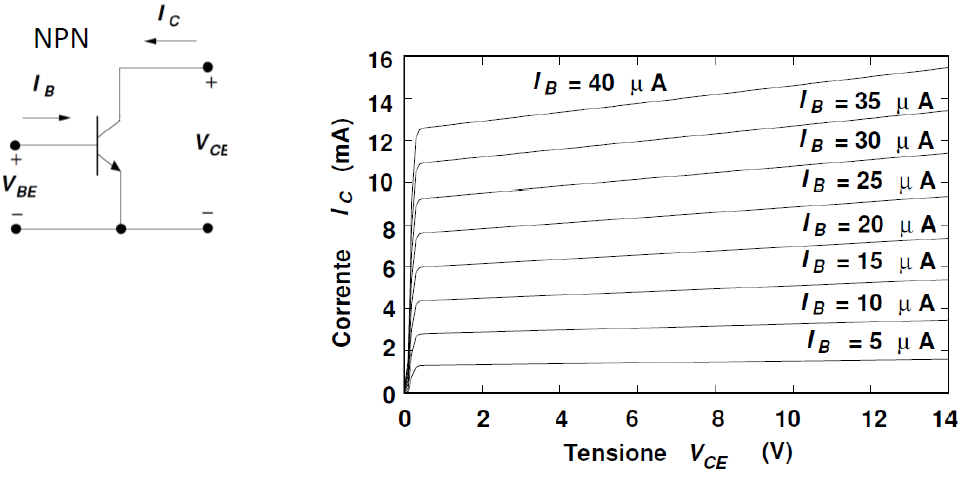
\includegraphics[width=0.5\linewidth]{img/eff early.png}
\end{figure}
Osservando un BJT a caratteristiche reali osserviamo che queste non sono perfettamente orizzontali, quindi $I_C$ aumenta all'aumentare di $V_{CE}$, e l'\textbf{effetto early}: rappresentando le caratteristiche in funzione di $V_{BE}$ e prolungando idealmente le caratteristiche secondo la loro inclinazione, vedo che si incontrano tutte ad una tensione negativa $V_A$ detta \textbf{tensione di Early}.
\begin{figure}[H]
    \centering
    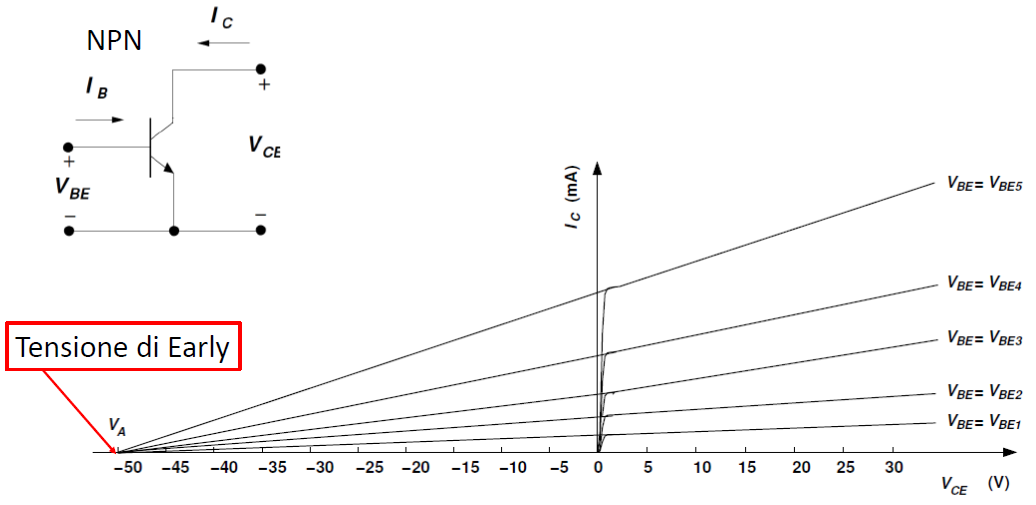
\includegraphics[width=0.5\linewidth]{img/tons early.png}
\end{figure}
Valori tipici di $V_A$ sono tra -50V e -100V: le caratteristiche non sono troppo inclinate.

L'origine di questo effetto è da ricercarsi nel modello fisico del transistore.
\subsection{Caratteristiche di un BJT PNP}
\begin{figure}[H]
    \centering
    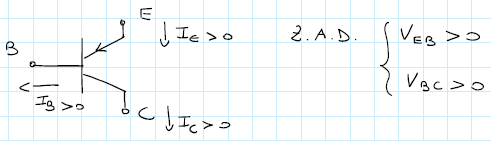
\includegraphics[width=0.5\linewidth]{img/car pnp.png}
\end{figure}

\section{I MOS - Metal Oxide Semiconductor}
\subsection{Transistori MOSFET}
Questi sono della famiglia dei Transistori a Effetto di Campo, ovvero dispositivi il cui funzionamento dipende da un campo elettrico.
Sono assimilabili a generatori di corrente controllati in tensione.
A differenza dei BJT\footnote{Dipendono dai portatori minoritari immessi in base} il loro comportamento dipende dei portatori maggioritari.
\begin{figure}
    \centering
    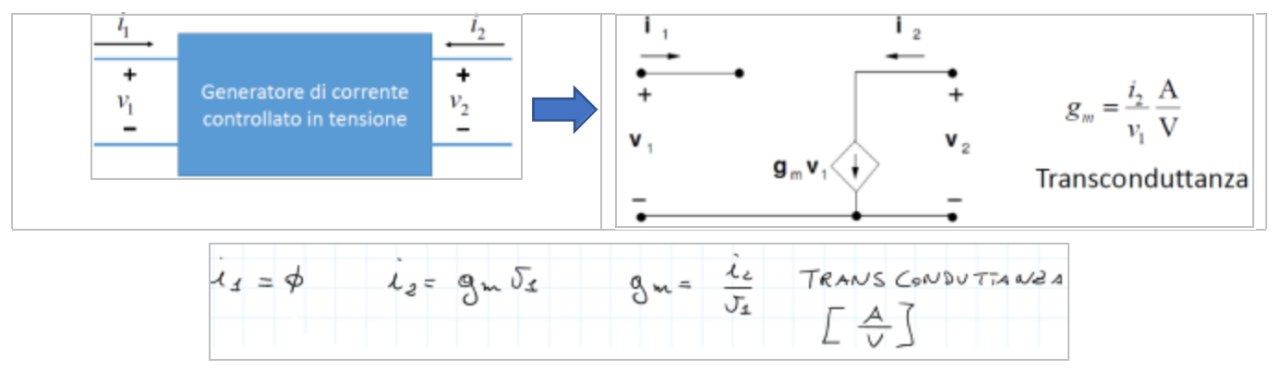
\includegraphics[width=0.5\linewidth]{img/schema mosfet.png}
    \caption{Schema circuitale}
\end{figure}
Notiamo come in ingresso abbiamo la tensione $V_1$ (terminale di controllo) e un'impedenza infinita, la corrente assorbita dal terminale di controllo è infatti nulla.
Nel terminale di uscita c'è $I_2=g_MV_1$ dove $g_M$ è il rapporto tra corrente di uscita e tensione in ingresso, è quindi una \textbf{trans-conduttanza} (rapporto tra grandezze di maglie diverse)
\subsection{Condensatore MOS}
Dispositivo osservabile come un condensatore con due armature, una di metallo e una di substrato, e il dielettrico con formula chimica $SiO_2$
\begin{figure}[H]
    \centering
    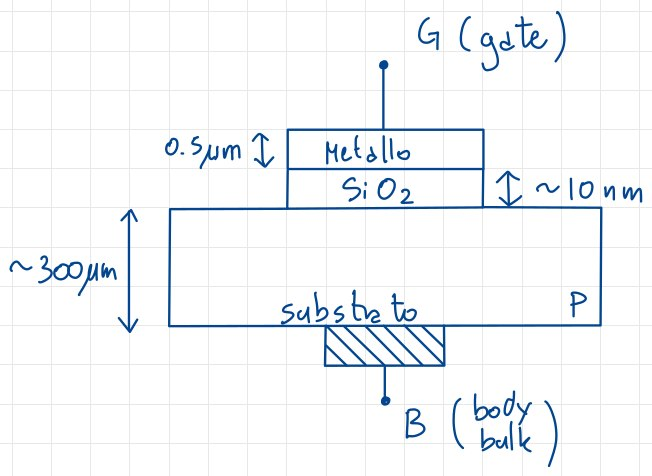
\includegraphics[width=0.5\linewidth]{img/cond mos.png}
\end{figure}
\begin{itemize}
    \item \textbf{substrato}: silicio drogato P
    \item \textbf{isolante}: ossido di silicio
    \item \textbf{metallo}: conduttore perfetto detto \textbf{gate}, sarà il terminale di controllo della corrente in uscita
\end{itemize}A seconda della tensione di gate $V_G$ che entra nel diodo avremo differenti comportamenti.
\subsubsection{Dispositivo in accumulazione}
$V_G<0$: il gate inizia a caricarsi negativamente, così il substrato lo fa positivamente, quindi campo elettrico che sposta (\textbf{accumulazione}) le lacune libere del substrato sulla zona superficiale (fermate dall'isolate).
\begin{figure}[H]
    \centering
    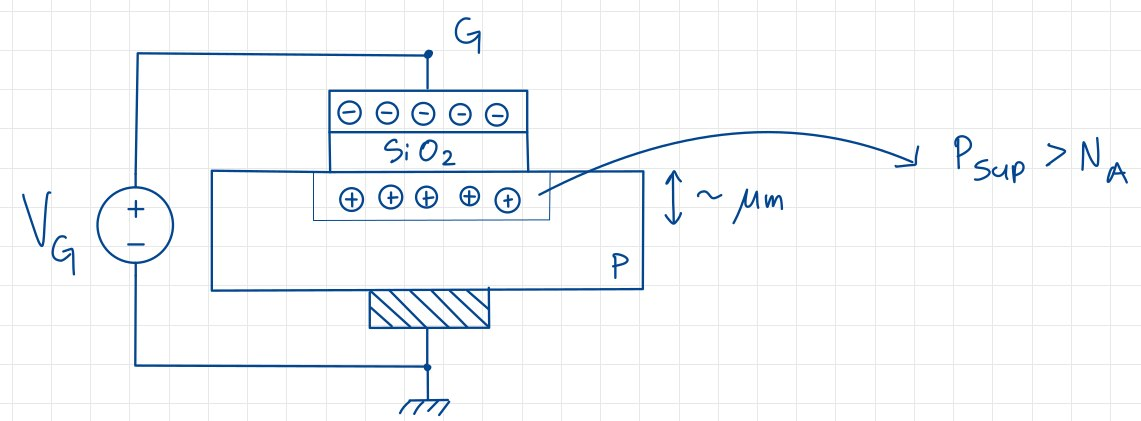
\includegraphics[width=0.5\linewidth]{img/disp in acc.png}
    \caption{Dispositivo in accumulazione}
\end{figure}
\subsubsection{Dispositivo in svuotamento}
Caso in cui tensione applicata al gate positiva ma minore di tensione di soglia $V_T$.
\begin{figure}[H]
    \centering
    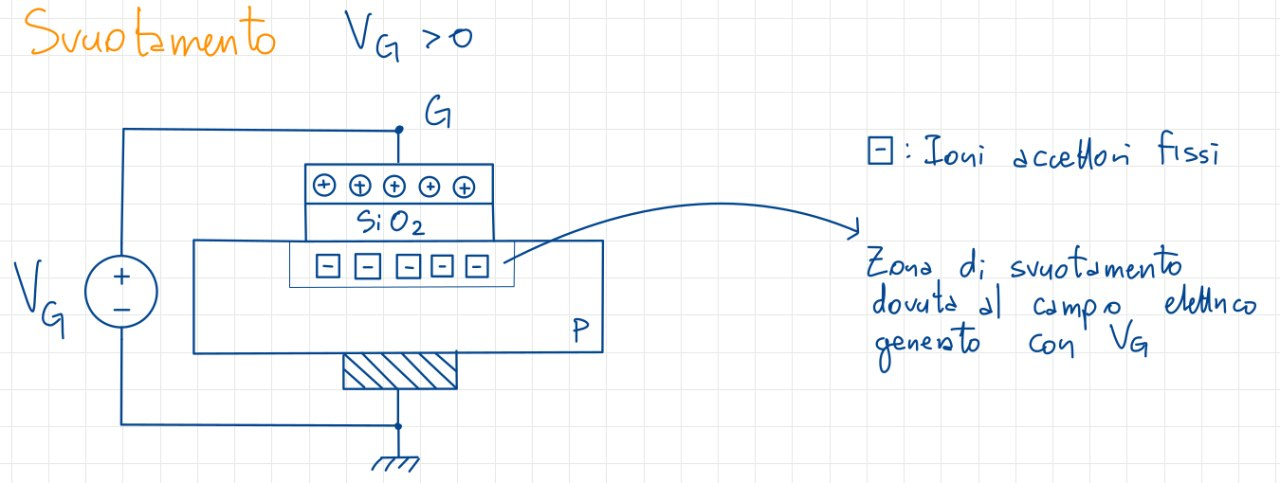
\includegraphics[width=0.5\linewidth]{img/disp svuot.png}
\end{figure}
In questo caso il campo elettrico che si genera allontana le lacune della superficie del substrato, si ha quindi una \textbf{zona di svuotamento}.
\subsubsection{Dispositivo di inversione}
Per tensioni sopra la soglia il campo elettrico allontana sempre di più le lacune attirando in superficie gli elettroni liberi del substrato P (minoritari, generati termicamente).
Questo accumulo andrà a compensare la carica positiva del gate, si ha quindi una \textbf{inversione locale}.
\begin{figure}[H]
    \centering
    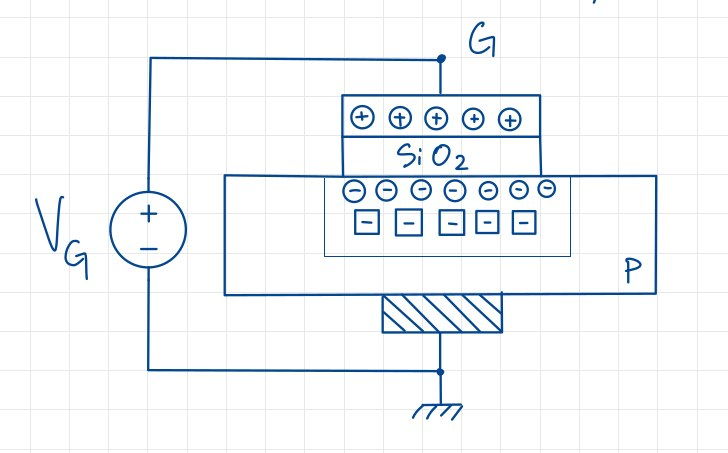
\includegraphics[width=0.5\linewidth]{img/disp inv.png}
\end{figure}
\subsection{MOSFET}
Condensatore MOS affiancato da due zone di semiconduttore con \textbf{drogaggio opposto a quello del body} (dette \textit{pozzetti})i cui terminali sono detti \textbf{source} e \textbf{drain}.
I pozzetti devono essere parzialmente sovrapposti all'ossido, la zona interposta tra i due pozzetti viene detta regione di canale (with lenght and width).

Il source è il terminale che fornisce i portatori, mentre drain li riceve; la corrente scorrerà da Source a Drain quando vengono rifornite lacune, mentre se vengono riforniti elettroni, la corrente scorrerà in senso opposto, e ciò viene regolato dalla tensione applicata su gate, che è il terminale di controllo del dispositivo.

Il terminale di body verrà messo a ground; schematizziamo inoltre le giunzioni $N+$ e $P$ come dei diodi che, per garantire il corretto funzionamento del dispositivo, devono essere in inversa (per garantirlo tensione in body la più piccola di tutto il circuito).

\subsubsection{MOSFET in accumulazione}
Applicando $V_{GS}<0$ si accumulano cariche positive nella superficie del substrato impedendo il passaggio di corrente da S a D.
\subsubsection{MOSFET in svuotamento}
Situazione opposta alla precedente, ci sono cariche fisse (-) che impediscono lo scorrere della corrente per $0<V_{GS}<V_T$.
\subsubsection{MOSFET in inversione}
$V_{GS}>V_T$ S e D collegati (prima erano isolati). Si verifica infatti lo stesso fenomeno dell'inversione visto nel MOS.
La differenza è che, nelle cariche mobili, gli elettroni generati termicamente sono una minima parte, a fronte delle cariche libere richiamate dalle regioni di S e D che fungono da \textbf{serbatoi di cariche}.
Sulla superficie del substrato si forma una zona con concentrazione di cariche libere, in questo caso elettroni, maggiore o uguale del drogaggio del substrato. Per effetto dell'inversione avremo che le due regioni $N^+$ sono unite da un canale conduttivo di cariche mobili, che permettono il passaggio di corrente. dando vita quindi a un MOSFET a canale N.
\begin{figure}[H]
    \centering
    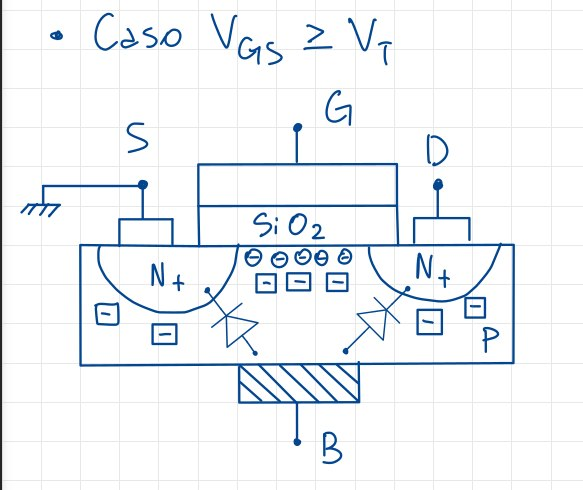
\includegraphics[width=0.5\linewidth]{img/mosfet inversione.png}
\end{figure}

\subsection{Studio del canale di un MOSFET}
Vediamo il comportamento del canale creato ($V_{GS}>V_T$).
\subsubsection{caso V\_DS > 0 e piccola}
S tensione di riferimento e D tensione positiva.
\begin{figure}[H]
    \centering
    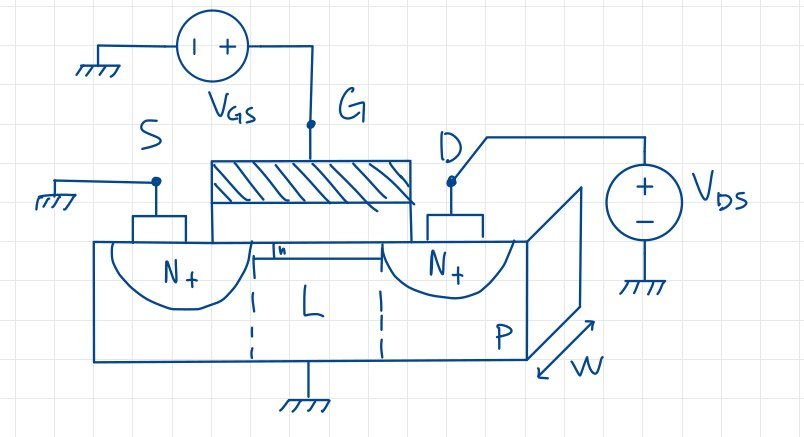
\includegraphics[width=0.5\linewidth]{img/mosfet pic.png}
\end{figure}
D inizia ad attrarre elettroni, quindi scorrimento di elettroni tra S e D (come suggerito dai nomi di questi elementi). 
...
\subsubsection{Caso per V\_DS>0 e non trascurabile}
In questo caso il canale non è più uniforme e cambia forma.
\begin{figure}[H]
    \centering
    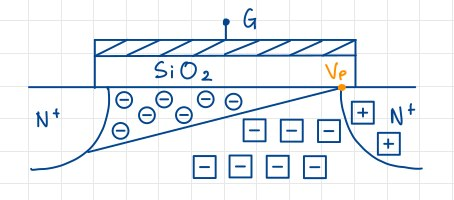
\includegraphics[width=0.25\linewidth]{img/cambio forma.png}
\end{figure}
\subsubsection{Strozzamento del canale}
Aumentando quella tensione il canale si strozza e si chiude: troviamo quindi la \textbf{tensione di strozzamento} o di \textbf{pinch-off}:
\[
V_{gS} = V_{GS} -V_T
\]
Se la $V_{DS}$ è maggiore di quella di strozzamento il canale si chiude in un punto precedente a drain.

\subsubsection{Conclusioni}

La corrente in un MOSFET si suddivide in due principali zone di funzionamento.

\paragraph{Zona di Triodo}

In questa regione, il canale è sempre \textbf{aperto} e la corrente $i_{DS}$ è influenzata sia dalla tensione gate-source ($V_{GS}$) che dalla tensione drain-source ($V_{DS}$). L'equazione che descrive la corrente in questa zona è:
$$i_{DS} = \mu_n \cdot C_{ox} \frac{W}{L} \left[ (V_{GS} - V_T) \cdot V_{DS} - \frac{V_{DS}^2}{2} \right]$$
\noindent dove:
\begin{itemize}
    \item $\mu_n$ è la mobilità dei portatori negativi;
    \item $C_{ox}$ è la capacità di ossido, data dal rapporto tra la costante dielettrica e lo spessore dell'ossido;
    \item $W$ è la larghezza del canale;
    \item $L$ è la lunghezza del canale.
\end{itemize}


\paragraph{Zona di Saturazione}

In questa regione, il canale del MOSFET è considerato \textbf{chiuso}. La corrente $i_{DS}$ dipende principalmente dalla tensione gate-source ($V_{GS}$) ed è quasi indipendente dalla tensione drain-source ($V_{DS}$). L'equazione della corrente diventa:
$$i_{DS} = \mu_n \cdot C_{ox} \frac{W}{L} \cdot \frac{(V_{GS} - V_T)^2}{Z}$$
Questa equazione è talvolta semplificata come $i_{DS} = k(V_{GS} - V_T)^2$, dove $k$ è una costante di proporzionalità.

\paragraph{Effetto Early}

Similmente a quanto accade nei transistori bipolari, anche nei MOSFET si manifesta un effetto noto come \textbf{Effetto Early}. Questo fenomeno causa una leggera inclinazione nelle curve di corrente in zona di saturazione, rendendo la corrente non perfettamente costante al variare di $V_{DS}$.

Per tener conto di questo effetto, l'equazione di saturazione viene modificata aggiungendo un fattore che dipende da $\lambda$:
$$i_{DS} = \mu_n \cdot C_{ox} \frac{W}{L} (V_{GS} - V_T)^2 (1 + \lambda v_{ds})$$
Prolungando le caratteristiche di saturazione, si nota che si incontrano in un punto del secondo quadrante chiamato $-\frac{1}{\lambda}$.
\subsubsection{La trans-caratteristica del MOSFET}
\subsection{Transistore MOSFET a canale P}
A differenza degli N-MOSFET sono caratterizzati da un substrato di tipo N (le diffusioni di S e D sono di tipo P).
\subsection{Cenni MOSFET a svuotamento}
I MOSFET visti finora sono detti ad arricchimento perché il canale viene costruito solo dopo l'applicazione di una certa tensione al gate.

\noindent In quelli a vuotamento invece il canale viene realizzato direttamente dal costruttore.
\subsection{Simboli circuitali di un MOSFET}
\begin{figure}[H]
    \centering
    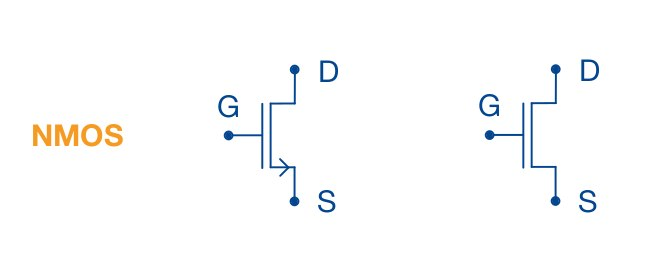
\includegraphics[width=0.5\linewidth]{img/msfet na n.png}
    \caption{A canale N}
\end{figure}
\begin{figure}[H]
    \centering
    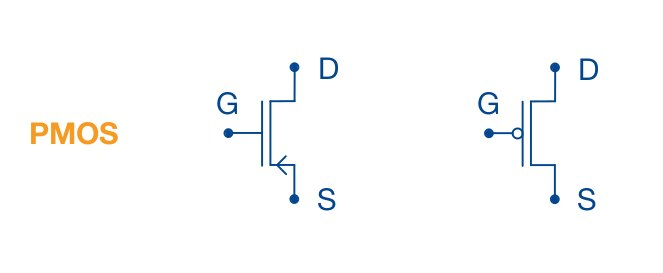
\includegraphics[width=0.5\linewidth]{img/msfte can p.png}
    \caption{A canale P}
\end{figure}

\section{Polarizzazione di transistori BJT}
\begin{definizione}
    [Polarizzare un circuito]
    La polarizzazione dei circuiti è l'operazione di applicare le opportune tensioni e correnti continue (DC) ai terminali di un componente elettronico attivo (come un transistor BJT o MOSFET) per portarlo in un punto di funzionamento specifico, chiamato anche punto di riposo o punto Q. Questo punto definisce le condizioni di lavoro del dispositivo in assenza di un segnale in ingresso variabile.
\end{definizione}
I transistori BJT hanno zone di funzionamento determinate dalla polarizzazione del dispositivo: per utilizzarli come amplificatore zona attiva diretta ovvero base-emettitore in diretta e base-collettore in inversa.
\subsection{Esempio circuito BJT}
\begin{figure}[H]
    \centering
    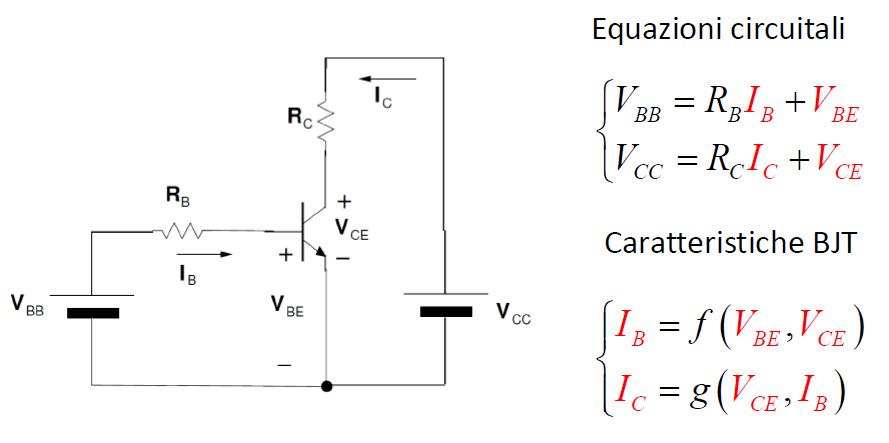
\includegraphics[width=0.75\linewidth]{img/circ sempl.png}
    \caption{Circuito BJT più semplice}
\end{figure}
2 porte in ingresso e 2 in uscita

\section{Polarizzazione di un MOSFET}

\section{I dispositivi come quadripoli}

\section{Gli amplificatori}
\begin{definizione}
    [Amplificatore]
    Dispositivo avente porta di ingresso e porta di uscita. Sono caratterizzati da parametri \textbf{di merito}.
    \begin{figure}[H]
        \centering
        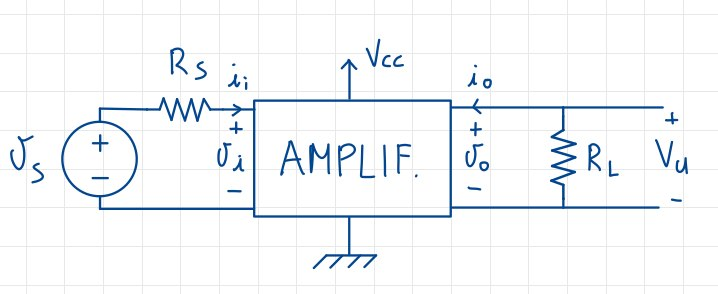
\includegraphics[width=0.5\linewidth]{img/amp.png}
        \caption{Schema generale di un amplificatore}
    \end{figure}
    I parametri di merito sono i seguenti:
    \begin{table}[H]
        \centering
        \begin{tabular}{cccc}
        \textbf{Guadagno di corrente} & \textbf{Guadagno di tensione} \\
        $A_i = \dfrac{i_{usc}}{i_{ing}}$ & $A_v = \dfrac{v_{usc}}{v_{ing}}$\\ 
         \textbf{Resistenza di ingresso} & \textbf{Resistenza di uscita} \\
         $R_{in} = \dfrac{v_{in}}{i_{in}}$ & $R_{out} = \dfrac{v_{out}}{i_{out}}$
        \end{tabular}
    \end{table}
\end{definizione}
\subsection{Circuito equivalente}
\begin{figure}[H]
    \centering
    \includegraphics[width=0.5\linewidth]{img/amp circ eq.png}
\end{figure}
\subsection{Analisi del circuito di un amplificatore}
L'analisi è divisa in due parti:
\begin{enumerate}
    \item Determinazione del punto di riposo (\textbf{analisi DC})
    \begin{enumerate}
        \item Disattivazione dei generatori del segnale (cortocircuiti per i generatori di tensione, apertura per i generatori di corrente)
        \item Sostituzione di condensatori e induttori rispettivamente con circuiti aperti e cortocircuiti
        \item Sostituzione dei componenti non lineari con il rispettivo modello per grandi segnali
    \end{enumerate}
    \item analisi del circuito equivalente sottoposto a segnali variabili nel tempo e con frequenza variabile. (\textbf{analisi a medie frequenze o analisi AC})
    \begin{enumerate}
        \item Disattivare i generatori di valore costante
        \item sostituire di condensatori e induttori rispettivamente con cortocircuiti e circuiti aperti
        \item sostituire i componenti non lineari nel rispettivo modello per piccole segnali, dipendentemente dal punto di riposo Q trovato
    \end{enumerate}
\end{enumerate}
\begin{nota}
    Per l'analisi DC sono fondamentali i manuali delle caratteristiche dei dispositivi, in quanto essi contengono già molti dati utili.
\end{nota}
\subsection{Amplificatore a emettitore comune}
\begin{figure}[H]
    \centering
    \includegraphics[width=0.4\linewidth]{img/amp em com.png}
\end{figure}
\begin{figure}[H]
    \centering
    \includegraphics[width=0.4\linewidth]{img/amp comp com.png}
    \caption{Circuito modificato in modo da evitare che il punto di riposo dipenda direttamente da R\_S}
\end{figure}
\subsubsection{Analisi AC}
Si ricava infine:
\[
A_{v} = \frac{v_{u}}{v_{s}} = - \frac{(R_{C} \parallel R_{L}) h_{fe}}{h_{ic} + R_{E} (h_{fe} + 1)}
\]
\noindent Considerazioni
\begin{enumerate}
    \item $A_v<0$ \textbf{configurazione invertente} (es. come uno sfasamento di 180 di una sinusoide)
    \item Se $R_E = 0 \to A_v = -\frac{(R_C||R_L)h_{fe}}{h_{ie}} \gg A_v \text{ con } R_E \neq 0$ ovvero l'aggiunta di $R_E$ (\textbf{resistenza di degenerazione di emettitore}) per la stabilizzazione del circuito fa diminuire il guadagno
    \item Se $R_E(h_{fe}+1) \gg h_{ie}$, allora $A_v = -\frac{R_C||R_L}{R_E}$ l'amplificazione non dipende più dalle caratteristiche del transistore ma solo dalle resistenze, dato che si possono scegliere il circuito è molto stabile
\end{enumerate}

\subsubsection{Condensatore di bypass}
Inseribile per aumentare il guadagno
\begin{figure}[H]
    \centering
    \includegraphics[width=0.5\linewidth]{img/cond byp.png}
\end{figure}

\subsubsection{Resistenza di uscita}
Rapporta tra tensione di uscita e corrente di uscita:
\[
R_0=\left.\frac{v_u}{i_0}\right|_{v_i=0}=0
\]
infatti si ha $i_b=0$.
\subsection{Amplificatore a collettore comune}
\begin{figure}[H]   
    \centering
    \includegraphics[width=0.5\linewidth]{img/amp coll com.png}
\end{figure}
\subsubsection{Resistenze di ingresso e uscita}
La resistenza di ingresso è identica a quello ad emettitore comune.
In uscita ho $R_o = \frac{h_{ie}}{h_{fe}+1}$
\subsubsection{Guadagno}
\[
A_v = \frac{v_u}{v_i} = \frac{(R_E || R_L)(h_{fe} + 1)}{h_{ie} + (R_E || R_L)(h_{fe} + 1)}
\]
\noindent Osservazioni:
\begin{enumerate}
    \item $A_v$ è positiva, per cui i segnali in ingresso ed uscita avranno lo stesso segno, ed è ciò che ci aspettiamo da una configurazione \textbf{non invertente};
    \item $A_v < 1$ sempre, per costruzione;
    \item Se $h_{ie} \ll (R_E || R_L)(h_{fe} + 1)$, allora $A_v \approx 1$. Questo caso è chiamato configurazione a \textbf{inseguitore di emettitore}, in quanto l'amplificazione è fatta con un fattore quasi unitario, grazie al quale l'uscita segue l'ingresso.
\end{enumerate}

\subsection{Amplificatore a source comune}
\begin{figure}[H]   
    \centering
    \includegraphics[width=0.5\linewidth]{img/amp source comune.png}
\end{figure}
\subsubsection{Parametri di guadagno}
\[
A_v = \frac{v_u}{v_i} = -(r_d || R_D || R_L)g_m
\]
Negativa quindi invertente.
\subsubsection{Parametri di resistenza}
In ingresso accade come visto prima, quindi $R_i= \frac{v_i}{i_i}\to\infty$.
In uscita si ha una situazione più complicata:
\subsubsection{Caso particolare}
Caso in cui $R_S\neq 0$ e $r_d\to\infty$:
\begin{figure}[H]
    \centering
    \includegraphics[width=0.25\linewidth]{img/caso part.png}
\end{figure}
Si ottiene il ricavo:
\[
A_v = \frac{v_u}{v_i} = -(R_D||R_L)g_m \frac{1}{1 + R_S g_m}
\]
La \textbf{resistenza di degenerazione di source} ($R_S$) porta una stabilizzazione del punto di riposo e una riduzione del guadagno.

\subsection{Amplificatore a drain in comune}
Qui il drain è utilizzato come terminale di riferimento, al contrario il terminale di entrata sarà il gate.
\begin{figure}
    \centering
    \includegraphics[width=0.5\linewidth]{img/amp drain com.png}
    \caption{Circuito simile al precedente, rimuoviamo R\_D}
\end{figure}
\subsubsection{Parametri di output}
\[
A_v = \frac{v_u}{v_i} = \frac{g_m((R_S||R_L))}{1+g_m((R_S||R_L))}
\]
Configurazione in esame sia \textbf{non invertente}, ciò è ravvisabile dal segno positivo di $A_v$; sempre osservando la relazione appena trovata ci accorgiamo che $|A_v| < 1$ per costruzione e che, nel caso particolare in cui $g_m((R_S||R_L)) \gg 1$, $A_v \approx 1$, configurazione che prende il nome di \textbf{inseguitore di source}.
\subsection{Amplificatori multistadio}
Combinare in cascata più amplificatori in modo da \textbf{combinare le loro caratteristiche} per soddisfare tutti i requisiti di un progetto.
\begin{figure}[H]
    \centering
    \includegraphics[width=0.25\linewidth]{img/es amp multistadio.png}
\end{figure}
\subsubsection{Interazione tra stadi}
Per capire come gli stadi interagiscono tra di loro esplicitiamo i loro circuiti equivalenti.
\begin{figure}[H]
    \centering
    \includegraphics[width=0.5\linewidth]{img/espli circ eq.png}
\end{figure}
\noindent Guadagno dato da
\[
A_v = A_{v1}A_{v2}\frac{R_{i2}}{R_{o1} + R_{i2}}
\]
dove $\frac{R_{i2}}{R_{o1} + R_{i2}}$ è detto fattore di attenuazione e per costruzione non può essere negativo o maggiore di 1.

Vale 1 solo quando $R_{i2}\to\infty$ o $R_{o1}=0$: in questo caso si dice che lo stadio a valle \textbf{insegue} lo stadio a monte.

\section{Risposta in frequenza}
Essendo un segnale, in genere, composto da più componenti frequenziali (spesso in forma sinusoidale) bisogna stare attenti, con gli amplificatori, ad amplificare tutte le componenti allo stesso modo per evitare \textbf{distorsione} del segnale originale.
\subsection{Determinazione della risposta in frequenza}
\begin{definizione}
    [Elementi reattivi]
    Elementi che determinano la risposta in frequenza.
    \begin{nota}
        Ad esempio elementi che dipendono dalla frequenza come induttori o condensatori.
    \end{nota}
\end{definizione}
Per determinare la risposta in frequenza ad esempio di $A_v$ dovrei calcolare tutti i poli e gli zeri del circuito per poi passare effettivamente alla risposta in frequenza.
Devo quindi prima portare il circuito nel dominio della frequenza: ogni condensatore inserisce uno zero nell'origine (a frequenze nulle sono assimilabili a dei circuiti aperti).
In un circuito, in genere, il numero di poli è pari al numero di \textbf{elementi reattivi indipendenti}.

\subsection{Ruolo dei condensatori}
Nell'analisi \textbf{DC} li considero \textbf{sempre} come \textbf{aperti}.

\noindent In \textbf{AC}:
\begin{itemize}
    \item a \textbf{basse frequenze} considero i condensatori interni come circuiti aperti;
    \item a \textbf{medie frequenze} considero i condensatori interni come circuiti aperti, e quelli esterni come cortocircuiti;
    \item ad \textbf{alte frequenze} considero i condensatori esterni come cortocircuiti.
\end{itemize}
\subsection{Diagramma di Bode}
\begin{figure}[H]
    \centering
    \includegraphics[width=0.5\linewidth]{img/bode amp.png}
    \caption{Diagramma di Bode generale per gli amplificatori}
\end{figure}
Notare inoltre $f_T$ ovvero frequenza di \textbf{transizione}, valore per il quale il guadagno di corrente in cortocircuito, nella configurazione ad emettitore comune, diventa unitaria.
\subsection{Utilizzi digitali di amplificatori e elementi attivi}
\begin{definizione}
    [Elemento attivo]
    Elemento che ha bisogno di alimentazione.
\end{definizione}
\subsubsection{Inverter}
\begin{figure}[H]
    \centering
    \includegraphics[width=0.4\linewidth]{img/inv.png}
\end{figure}
\begin{figure}[H]
    \centering
    \includegraphics[width=0.3\linewidth]{img/car trasf invert.png}
    \caption{Caratteristica di trasferimento dell'inverter}
\end{figure}
\subsubsection{Inverter con BJT}
\begin{figure}[H]
    \centering
    \includegraphics[width=0.3\linewidth]{img/inv bjt.png}
\end{figure}

\subsection{Teoria della reazione semplificata}
\begin{definizione}
    [Principio della reazione]
    Consiste nel riportare all'ingresso di un sistema una porzione del segnale in uscita dallo stesso, in modo da modificare le proprietà del sistema stesso. Generalmente, nei casi nei quali è necessario mantenere una grandezza in uscita costante, si parla, e si realizza, una reazione negativa, ovvero che il segnale riportato in ingresso ha segno inverso rispetto al segnale che lo ha prodotto: così facendo ogni variazione determina un effetto in senso opposto, che tende a contrastare la variazione stessa. Questo tipo di reazione è quella che viene maggiormente utilizzata in campo elettronico, visto il bisogno di generare tensioni e correnti stabili.
\end{definizione}
\begin{figure}
    \centering
    \includegraphics[width=0.5\linewidth]{img/schema gen segn rettr.png}
    \caption{Schema generale di un sistema retroazionato}
\end{figure}

\section{Amplificatori Differenziali}
\begin{definizione}
    [Amplificazione differenziale]
    Tipo di amplificatore che, dati due segnali tramite due porte di ingresso, produce in uscita un segnale che è l'amplificazione della differenza tra i due segnali in ingresso moltiplicata per un fattore di amplificazione.
    \begin{figure}[H]
        \centering
        \includegraphics[width=0.25\linewidth]{img/ampl diff.png}
    \end{figure}
\end{definizione}
\begin{definizione}
    [Segnale a modo differenziale]
    Il segnale a modo \textbf{differenziale} $v_d$ è quel segnale dato dalla \textbf{differenza} tra i due segnali in ingresso $v_1$ e $v_2$.
\end{definizione}
\begin{definizione}
    [Segnale a modo comune]
    Il segnale a modo \textbf{comune} $v_c$ è la \textbf{semisomma} dei due segnali in ingresso $v_1$ e $v_2$.
\end{definizione}
\begin{definizione}
    [Guadagno del modo differenziale]
    Il \textbf{guadagno del modo differenziale} $A_d$ è il rapporto tra il segnale a modo differenziale $v_d$ e il segnale in uscita $v_u$, ovvero: $A_d = \frac{v_u}{v_d}$.    
\end{definizione}
\begin{definizione}
    [Guadagno del modo comune]
    Il \textbf{guadagno del modo comune} $A_c$ è il rapporto tra il segnale in uscita $v_u$ e il segnale a modo comune $v_c$, ovvero: $A_c = \frac{v_u}{v_c}$.    
\end{definizione}

\subsection{Caso reale e caso ideale}
Se abbiamo dei disturbi sui segnali in ingresso all'amplificatore, essi tenderanno ad eliminarsi se questi sono uguali. In caso reale, tuttavia, è impossibile che i due disturbi siano identici.

\subsection{Amplificatori operazionali}
Sono una tipologia di amplificatori differenziali, inizialmente utilizzati per fare operazioni tra segnali.
\begin{figure}
    \centering
    \includegraphics[width=0.4\linewidth]{img/amp op.png}
\end{figure}
dove i segni + e - indicano l'ingresso \textbf{non invertente} e quello \textbf{invertente}.

\subsection{Circuito sommatore}
Si tratta di un amplificatore operazionale invertente
\begin{figure}[H]   
    \centering
    \includegraphics[width=0.5\linewidth]{img/circ somma.png}
\end{figure}
\subsection{Circuito sottrattore}
Questo circuito possiede una novità: ha una configurazione che è un misto tra una invertente e una non invertente. L'obiettivo è quello di amplificare tensioni anche quando esse non sono piccole (ricordiamo il caso reale del differenziale). Vorremo dunque che l'uscita di questo circuito sia uguale, a meno di una costante moltiplicativa, alla differenza tra i due segnali in ingresso.
\begin{figure}[H]
    \centering
    \includegraphics[width=0.5\linewidth]{img/circ sott.png}
\end{figure}
\subsection{Integratore di Miller}
Questo circuito è un amplificatore operazionale invertente, con un condensatore in retroazione.
\begin{figure}[H]
    \centering
    \includegraphics[width=0.5\linewidth]{img/amp miller.png}
\end{figure}

\section{I regolatori}
Riaffrontiamo i regolatori \textbf{di tensione} avvalendoci però degli amplificatori di tensione.
Introduciamo anche regolatori \textbf{di corrente} e \textbf{altri}.
\begin{nota}
    [Reminder sui regolatori di tensione]
    dispositivo che, dato in ingresso una certa tensione sinusoidale (o comunque non costante), restituisce in uscita una tensione costante, indipendente dal carico.
\end{nota}
\begin{nota}
    [Limiti dei dispositivi con diodo zener]
    $\s$
    \begin{itemize}
        \item corrente in uscita non perfettamente costante
        \item limite di potenza
    \end{itemize}
\end{nota}
\subsection{Regolatore di tensione ideale}
Circuito elettronico che produce in uscita una tensione \textbf{continua} e \textbf{indipendente} da:
\begin{enumerate}
    \item la \textbf{corrente di carico} $I_L$;
    \item la \textbf{tensione di ingresso} $V_{in}$;
    \item la \textbf{temperatura} $T$.
\end{enumerate}
\subsection{Regolatore di tensione lineare serie}
\subsubsection{Circuito con diodo Zener}
\begin{figure}[H]
    \centering
    \includegraphics[width=0.5\linewidth]{img/circ ocn did zen.png}
\end{figure}
\begin{nota}
    $R_S$ deve essere molto grande per evitare la rottura del diodo Zener.
\end{nota}
\subsubsection{Circuito con amplificatore}
Qui si ha una reazione in tensione grazie all'amplificatore.
\begin{figure}[H]
    \centering
    \includegraphics[width=0.5\linewidth]{img/circ con amp reg.png}
\end{figure}
\subsection{Limitazioni in frequenza}
Osservando l'equivalente di Tevenin del circuito si ha che bisogna aggiungere un condensatore: questo funge da filtro passa basso.
\subsection{Regolatori di corrente}
\subsubsection{Componente 78XX}
\begin{figure}[H]
    \centering
    \includegraphics[width=0.25\linewidth]{img/78xx.png}
\end{figure}
\paragraph{Problemi del circuito}
Ci sono due problemi principali che si possono incorntrare:
\begin{itemize}
    \item sono \textbf{poco flessibili}, per cui se voglio cambiare alcuni valori o parametri devo \textbf{riprogettare tutto il sistema};
    \item viene dissipata \textbf{molta tensione} sotto forma di calore, che porta ad un \textbf{basso rendimento}.
\end{itemize}
\noindent Per questo motivo si preferisce utilizzare un \textbf{regolatore switching}.
\subsection{Regolatori switching (a commutazione non lineare)}
Dato che il problema precedente era la dissipazione di energia si parte dall’elemento circuitale che per definizione non dissipa energia: l’interruttore (o switch).
\begin{figure}[H]
    \centering
    \includegraphics[width=0.5\linewidth]{img/reg switch.png}
    \caption{Circuito con interruttore e tensione di uscita}
\end{figure}
\begin{definizione}
    [Duty cycle]
    Rapporto tra il tempo in cui l'interruttore è chiuso e il periodo di commutazione.
    \[
    D=\frac{T_{ON}}{T_S}
    \]
\end{definizione}
Il valore medio dell'uscita è proporzionale al duty cycle.
\subsubsection{Regolatore forward}
\begin{figure}[H]
    \centering
    \includegraphics[width=0.5\linewidth]{img/reg fw.png}
\end{figure}
\begin{nota}
    Filtro passa basso necessario per estrarre il valor medio del segnale senza dissipare energia.
\end{nota}
\paragraph{Dimensionamento del filtro}
Il corretto funzionamento del circuito dipende dal corretto funzionamento e dimensionamento del filtro.
Dal diagramma di Bode notiamo che il filtro scende di 40dB per decade e che l'interruttore ha frequenza $f_S$: è dunque necessario che $f_O<<f_S$ dove $f_O$ è la frequenza di taglio (dove il guadagno nel grafico inizia a scendere).
\subsubsection{Regolatore flyback}
Permette di ottenere in uscita una tensione che sia maggiore, minore o uguale a quella in ingresso.
\begin{figure}[H]
    \centering
    \includegraphics[width=0.5\linewidth]{img/reg flyback.png}
\end{figure}
\subsubsection{Isolamento galvanico}
\begin{figure}[H]
    \centering
    \includegraphics[width=0.5\linewidth]{img/chem imp.png}
    \caption{Schema ideale impianto casalingo}
\end{figure}
Essendo il trasformatore ingombrante e pesante, potremmo pensare di rimuoverlo e alimentare i dispositivi a tensione di rete; questo è però pericoloso in quanto viene a mancare l'\textbf{isolamento galvanico}, ovvero la connessione diretta tra rete e circuito interno (ciò che ci protegge dalla \textit{scossa}).
\subsection{Regolatori di tensione con trasformatore}
Analizziamo alcuni circuiti che fungono da regolatori di tensione.
\subsubsection{Regolatore forward con trasformatore in alta frequenza}
\begin{figure}[H]
    \centering
    \includegraphics[width=0.5\linewidth]{img/reg fow con t in freq.png}
\end{figure}
\subsubsection{Regolatore flyback con trasformatore in alta frequenza}
\begin{figure}[H]
    \centering
    \includegraphics[width=0.5\linewidth]{img/reg flyb con tr.png}
\end{figure}
\subsection{Regolatore switching flyback completo con circuito di regolazione}
\begin{figure}[H]
    \centering
    \includegraphics[width=0.75\linewidth]{img/mega circuito.png}
\end{figure}

\section{Circuiti digitali}
Introduciamo ora la parte di elettronica digitale, ovvero quella parte di elettronica che si occupa di circuiti che operano con segnali digitali.
\subsection{Il segnale digitale}
Un segnale digitale è una sequenza finita di numeri, dove ognuno di essi rappresenta l'ampiezza del segnale in un dato istante temporale. É quindi necessario individuare un sistema numerico per rappresentare i valori del segnale: nel caso dei circuiti digitali viene in aiuto in sistema binario, in quanto è possibile rappresentare i valori del segnale con due soli numeri, 0 e 1: associamo al valore 0 il valore di tensione più basso, e al valore 1 il valore di tensione più alto.
\begin{itemize}
    \item $0 \equiv [V_{LMAX} \div V_{LMIN}]$ (Voltage Low)
    \item $1 \equiv [V_{HMAX} \div V_{HMIN}]$ (Voltage High)
\end{itemize}
\begin{nota}
    In realtà associamo un insieme di valori per far fronte a rumori e disturbi.
\end{nota}
\subsection{Le tecnologie usate}
\subsubsection{Inverter come esempio di circuito digitale}
\begin{figure}[H]
    \centering
    \includegraphics[width=0.5\linewidth]{img/inv dig.png}
\end{figure}
\begin{itemize}
    \item $V_{OHMIN}$ è il valore minimo per avere in uscita 1 (Output HIgh), $V_{IHMIN}$ corrispondente tensione in ingresso
    \item $V_{IHMIN}$ corrispondente tensione in ingresso
    \item $V_{OLMAX}$ è il valore massimo per avere in uscita 0 (Output Low), 
    \item $V_{ILMIN}$ corrispondente tensione in ingresso
\end{itemize}
Questi sono i punti in cui $|\frac{\partial v_O}{\partial v_I}|=1$.

\subsection{Caratteristiche dei circuiti digitali}
\subsection{Inverter CMOS}
Questa innovativa configurazione prevede l'uso di un PMOS e di un NMOS, utilizzati rispettivamente per gli ingressi alti e bassi. 
L'idea di base è realizzare un circuito che abbia due interruttori in controfase, ovvero interruttori mai attivi contemporaneamente, in modo da avere una potenza statica dissipata nulla.
\subsubsection{Circuito}
\begin{figure}[H]
    \centering
    \includegraphics[width=0.25\linewidth]{img/in cmos.png}
\end{figure}


\section{Circuiti logici}

\section{Logica sequenziale}




\end{document}